\documentclass[11pt,a4paper,twoside,openright]{book}
%\documentclass[tikz,border=10pt]{article}

\usepackage{url,amsfonts,epsfig}
\usepackage{afterpage}
\usepackage{amsmath,amssymb}            
\usepackage{rotating}  
\usepackage{fancyhdr}  

%\usepackage[scriptsize]{caption2} 
%\hyphenation{a-gen-tiz-za-zio-ne}

%\setlength{\paperwidth}{16cm}
%\setlength{\paperheight}{24cm}
%\setlength{\oddsidemargin} {2. cm}
%\setlength{\evensidemargin} {2. cm}
\addtolength{\oddsidemargin} {-0.4 cm}
\addtolength{\evensidemargin} {-0.4 cm}
\linespread{1.1}
\usepackage[italian]{babel}
%\usepackage[latin1]{inputenc}
%\renewcommand{\captionfont}{\normalfont \sffamily \itshape \small}

\pagestyle{empty}

\usepackage{lmodern}
\usepackage{amssymb,amsmath}
\usepackage{ifxetex,ifluatex}
\usepackage{fixltx2e} % provides \textsubscript
\usepackage{framed}

% Abs
\usepackage{mathtools,etoolbox}
\DeclarePairedDelimiterX{\abs}[1]{\lvert}{\rvert}{\ifblank{#1}{{}\cdot{}}{#1}}
\DeclarePairedDelimiter\ceil{\lceil}{\rceil}
\DeclarePairedDelimiter\floor{\lfloor}{\rfloor}

% Tables 
\usepackage{multirow}
\usepackage[table,xcdraw]{xcolor}
\newcommand{\specialcell}[2][c]{%
  \begin{tabular}[#1]{@{}c@{}}#2\end{tabular}}

% Trees
\usepackage{graphviz}
\usepackage{tikz}
\usetikzlibrary{arrows}
\tikzset{
  treenode/.style = {align=center, inner sep=0pt, text centered,font=\sffamily},
  arn_n/.style = {treenode, circle, white, font=\sffamily\bfseries, draw=black,
    fill=black, text width=1.5em},% arbre rouge noir, noeud noir
  arn_r/.style = {treenode, circle, red, draw=red, 
    text width=1.5em, very thick},% arbre rouge noir, noeud rouge
  arn_x/.style = {treenode, rectangle, draw=black,
    minimum width=0.5em, minimum height=0.5em}% arbre rouge noir, nil
}

% Graphs
\usepackage{float}
\usetikzlibrary{graphdrawing}
\usetikzlibrary{graphs}
\usegdlibrary{trees}

%other

\newcommand\myworries[1]{\textcolor{red}{#1}}

\usepackage{amssymb}
\usepackage{pgfgantt}

%code
% Code blocks
\usepackage{listings}
\usepackage{color} 
\definecolor{codegreen}{rgb}{0,0.6,0}
\definecolor{codegray}{rgb}{0.5,0.5,0.5}
\definecolor{codepurple}{rgb}{0.58,0,0.82}
\definecolor{backcolour}{rgb}{0.95,0.95,0.92}
\lstdefinelanguage{pseudocode}{
	sensitive=false,
	keywords={}
	otherkeywords={<,<=,>,>=,==,=, <-,->, !=}, %operators
	keywords=[2]{for, to, downto, foreach, while, if, else, then, do, return, repeat, until, and, or, in},
	keywords=[3]{true, false, nil, null},
	keywordstyle=\color{black},
	keywordstyle=[2]\color{blue},
	keywordstyle=[3]\color{red},
	comment=[l]{//},
	commentstyle=\color{grey},
	stringstyle=\color{red},
	numberstyle=\scriptsize
	%numberstyle=\tiny
}

\lstdefinestyle{pseudocodestyle}{
	language=pseudocode,
    backgroundcolor=\color{backcolour},   
    commentstyle=\color{codegreen},
    keywordstyle=\color{magenta},
    numberstyle=\tiny\color{codegray},
    stringstyle=\color{codepurple},
    basicstyle=\footnotesize,
    breakatwhitespace=false,         
    breaklines=true,                 
    captionpos=b,                    
    keepspaces=true,                 
    numbers=left,                    
    numbersep=5pt,                  
    showspaces=false,                
    showstringspaces=false,
    showtabs=false,                  
    tabsize=2,
    mathescape=true,
    frame=lrtb
}
\lstset{style=pseudocodestyle}


%style
\ifnum 0\ifxetex 1\fi\ifluatex 1\fi=0 % if pdftex
  \usepackage[T1]{fontenc}
  \usepackage[utf8]{inputenc}
\else % if luatex or xelatex
  \ifxetex
    \usepackage{mathspec}
  \else
    \usepackage{fontspec}
  \fi
  \defaultfontfeatures{Ligatures=TeX,Scale=MatchLowercase}
\fi
% use upquote if available, for straight quotes in verbatim environments
\IfFileExists{upquote.sty}{\usepackage{upquote}}{}
% use microtype if available
\IfFileExists{microtype.sty}{%
\usepackage[]{microtype}
\UseMicrotypeSet[protrusion]{basicmath} % disable protrusion for tt fonts
}{}
\PassOptionsToPackage{hyphens}{url} % url is loaded by hyperref
\usepackage[unicode=true]{hyperref}
\hypersetup{
            pdfborder={0 0 0},
            breaklinks=true}
\urlstyle{same}  % don't use monospace font for urls
\usepackage{longtable,booktabs}
% Fix footnotes in tables (requires footnote package)
\IfFileExists{footnote.sty}{\usepackage{footnote}\makesavenoteenv{long table}}{}
\usepackage{graphicx,grffile}
\makeatletter
\def\maxwidth{\ifdim\Gin@nat@width>\linewidth\linewidth\else\Gin@nat@width\fi}
\def\maxheight{\ifdim\Gin@nat@height>\textheight\textheight\else\Gin@nat@height\fi}
\makeatother
% Scale images if necessary, so that they will not overflow the page
% margins by default, and it is still possible to overwrite the defaults
% using explicit options in \includegraphics[width, height, ...]{}
\setkeys{Gin}{width=\maxwidth,height=\maxheight,keepaspectratio}
\IfFileExists{parskip.sty}{%
	\usepackage{parskip}
}{% else
	\setlength{\parindent}{0pt}
	\setlength{\parskip}{6pt plus 2pt minus 1pt}
}

\setlength{\emergencystretch}{3em}  % prevent overfull lines
\providecommand{\tightlist}{\setlength{\itemsep}{0pt}\setlength{\parskip}{0pt}}
\setcounter{secnumdepth}{0}

% Redefines (sub)paragraphs to behave more like sections
 \ifx\paragraph\undefined\else
\let\oldparagraph\paragraph
\renewcommand{\paragraph}[1]{\oldparagraph{#1}\mbox{}}
\fi
\ifx\subparagraph\undefined\else
\let\oldsubparagraph\subparagraph
\renewcommand{\subparagraph}[1]{\oldsubparagraph{#1}\mbox{}}
\fi

% set default figure placement to htbp
\makeatletter
\def\fps@figure{htbp}
\makeatother


\title{Appunti di Algoritmi e strutture dati}
\author{Filippo Bisconcin}
\date{2018}

\begin{document}

\frontmatter

\begin{titlepage}
\maketitle
\end{titlepage}

\pagestyle{plain}
\tableofcontents
\pagestyle{empty}\cleardoublepage
\pagenumbering{arabic}

\pagestyle{fancy} 
\fancyfoot{}                                               
\renewcommand{\chaptermark}[1]{\markboth{\chaptername\ \thechapter.\ #1}{}} 
\renewcommand{\sectionmark}[1]{\markright{\thesection.\ #1}}         
\fancyhead[LE,RO]{\bfseries\thepage}    
                                        
\fancyhead[RE]{\bfseries\leftmark}    
\fancyhead[LO]{\bfseries\rightmark}     
\renewcommand{\headrulewidth}{0.3pt} 

\mainmatter

%mod 1
\chapter{Algoritmi e loro complessità: i numeri di Fibonacci}

{~{[}DFI{]} cap. 1}

\begin{equation}
f(n) = 
\begin{cases}
1 & \mbox{se } n=1,n=2 \\ 
(n-1)+f(n-2) & \mbox{se } n\geq3 
\end{cases}
\end{equation}

\section{Formula di Binet}

\begin{equation}
\forall n \in N, F_n = \frac{1}{\sqrt{5}}(\Phi^n-\overline{\Phi}^n)
\end{equation}

Dove con $\Phi$ si indica la sezione aurea $\frac{1+\sqrt{5}}{2} \simeq -0,618$ e con $\overline{\Phi}$ si indica $\frac{1-\sqrt{5}}{2} \simeq -0,618$

\subsubsection{Dimostrazione}

{Dimostriamo per Induzione la formula di Binet:}

{Base:}

{$n = 1 \rightarrow F_n = \frac{1}{\sqrt{5}}(\Phi^1-\overline{\Phi}^1)$

{Sostistuisco con le definizioni di $\Phi$ e semplifico}

{$F_n = 1 = F_1$}

{$n = 2 \rightarrow F_n =\frac{1}{\sqrt{5}}(\Phi^2-\overline{\Phi}^2)$

{Sostistuisco con le definizioni di $\Phi$ e semplifico}

{$F_n = 1 = F_2$}

{Passo induttivo $n \geq 3$ :}

$F_n = F_{n-1} + F_{n-2}$

$F_{n-1}=\frac{1}{\sqrt{5}}(\Phi^{n-1}-\overline{\Phi}^{n-1})$ e 
$F_{n-2}=\frac{1}{\sqrt{5}}(\Phi^{n-2}-\overline{\Phi}^{n-2})$

{assomiglia alla forma $F_n=\frac{1}{\sqrt{5}}(\Phi^n-\overline{\Phi}^n)$}

{ci chiediamo se $\Phi^n=\Phi^{n-1}+\Phi^{n-2}$ e se $\overline{\Phi}^n=\overline{\Phi}^{n-1}+\overline{\Phi}^{n-2}$

{divido da entrambe le parti per $\Phi^{n-2}$ e $\overline{\Phi}^{n-2}$}

\paragraph{Definizione 1}

{Utilizzeremo la notazione $T_n$ per indicare la velocità/complessità di una particolare funzione (numero di righe di codice eseguite) }

\lstinputlisting{code/fib1.txt}

$T(Fib1)_n = 1\,\forall n$

{Problema: con l'aumentare di $n$, la funzione $Fib1(n)$ diventa sempre più imprecisa}

$Fib1_3=1,9999.. \simeq 2$ \\
$Fib1_{16}=986,699.. \simeq 987$ \\
$Fib1_{18}=2583,1.. \simeq 2584$

\paragraph{Definizione 2}

\lstinputlisting{code/fib2.txt}

\begin{equation}
T(Fib2)_n = 
\begin{cases}
1 & \mbox{se } n=1,n=2 \\ 
2 + T_{n-1} + T_{n-2} & \mbox{se } \forall n \geq 3 
\end{cases}
\end{equation}

{$T(Fib2)_n$ è una formula ricorsiva o ricorrenza}


\begin{tabular}{|c|c|}
\hline 
$n$ & $T_n$ \\ 
\hline 
1 & 1 \\ 
\hline 
2 & 1 \\ 
\hline 
3 & 2+1+1 = 4 \\ 
\hline 
4 & 2+4+1=7 \\ 
\hline 
5 & 2 + 7 + 4 = 13 \\ 
\hline 
\end{tabular} 

{Risolviamo la ricorrenza per determinare la complessità / bontà della funzione esaminata.}

\begin{itemize}
\tightlist
\item
  {andamento esponenziale rispetto ad $n$: funzione NON efficiente}
\item
  {andamento logaritmico / proporzionale rispetto ad $n$: funzione
  efficiente}
\end{itemize}

\begin{center}\rule{0.5\linewidth}{\linethickness}\end{center}

\subsubsection{Strumento 1 - Albero di ricorsione}

{Notiamo che $T(Fib2)_5=(1*5)+(2*4)=13$, dove $(1 * 5)$ è la complessità delle foglie (5 foglie con peso 1) e $(2 * 4)$ è la complessità dei nodi interni (4 nodi con peso 2)}

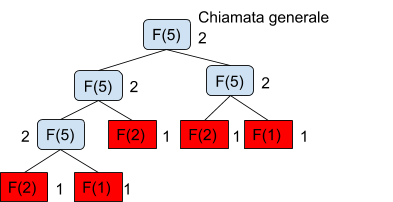
\includegraphics{images/image523.png}



\paragraph{Proprietà 1}

{Se $T_n$ rappresenta l'albero di ricorsione relativo a $Fib2_n$, allora il numero di foglie di $T_n$ è uguale a $F_n$(con $F_n$ indichiamo l'n-esimo numero della successione di Fibonacci)}

{Dimostrazione per induzione}

{Base:}

{se $n = 1$, il numero di foglie di $T_2$, $F_1=1$}

{se $n = 2$, il numero di foglie di $T_2$, $F_2=1$}

{Passo induttivo:}

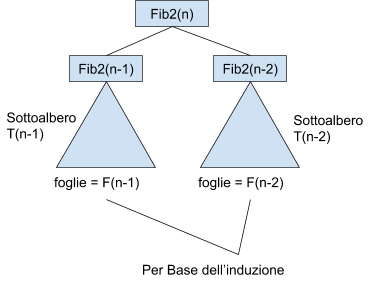
\includegraphics{images/image528.png}

\paragraph{Proprietà 2}

{Sia $T$ un albero binario in cui ogni nodo interno ha esattamente 2 figli}

{Allora $i_T=f_T-1$, dove con $i_T$ indichiamo il numero di nodi interni dell'albero $T$ e con $f_T$ indichiamo il numero di foglie dell'albero $T$}

\paragraph{Dimostrazione per induzione}

{Dimostrazione su $n$, dove $n$ è il numero di nodi di $T$}

{Base $n=1$ : OVVIO}

{Passo induttivo: $n \geq 2$}

{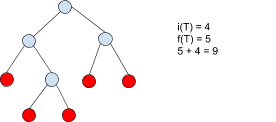
\includegraphics{images/image525.png}}

{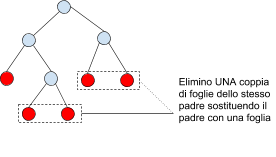
\includegraphics{images/image536.png}}

{L'albero risultante lo chiamiamo $\overline{T}$:}

{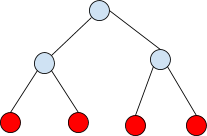
\includegraphics{images/image522.png}}

{Notiamo che }

$t_{\overline{T}} = f_{\overline{T}}-1${*}

$f_{\overline{T}} = f_{T}-1${**}

$i_{\overline{T}} = i_{T}-1$

{→ (inverto) $i_T=i_{\overline{T}}+1$}

{→ (sostituisco*) $i_T=f_{\overline{T}}+1-1$}

{→ (semplifico) $i_T=f_{\overline{T}}$}

{→ (sostituisco**) $i_T=f_T-1$}

{Studio complessità di $Fib2_n$ con l'utilizzo del metodo dell'albero di ricorsione}

$i_{T_n}=F_n-1$

$f_{T_n}=F_n$

$T_n = 2 * i_{T_n}+1*f_{T_n}$

{→ $2 * F_{n-1} + F_n$}

{→ $3 * F_n - 2$}

\paragraph{Proprietà 3}

\begin{equation}
\forall n \geq 6 \rightarrow F_n \geq 2^{\frac{n}{2}}
\end{equation}

{Dimostrazione per induzione}

{Base $n=6$ :}

$F_6=8$	\\
$2^{\frac{6}{3}}=2^3=8$

{Passo induttivo $n \geq 7$ :}

$F(n) \geq 2^{\frac{n-1}{2}} + 2^{\frac{n-2}{2}}$

$F(n) \geq 2^{\frac{n}{2}} * 2^{-\frac{1}{2}} + 2^{\frac{n}{2}} * 2^{-1} $

$F(n) \geq 2^{\frac{n}{2}} * ( 2^{-\frac{1}{2}} + 2^{-1} )$

{$2^{-\frac{1}{2}}+2^{-1}$ è sempre maggiore o uguale ad 1}

{$Fib2(n)$ risulta essere troppo poco efficiente}

$T(8)=61$

$T(45) = 3,404,709,508$

{Definiamo allora $Fib3(n)$ utilizzando l'iterazione al posto della ricorsione}

\lstinputlisting{code/fib3.txt}

$T(Fib3_n)=3+(n-2)+(n-1)=2n$

{Ci chiediamo se fib3 sia efficiente dal punto di vista della
memoria\ldots{}}


\chapter{Notazione asintotica: le classi O, \Omega, \Theta}

{{[}DFI{]} 2.2; {[}CLRS{]} 3.1}

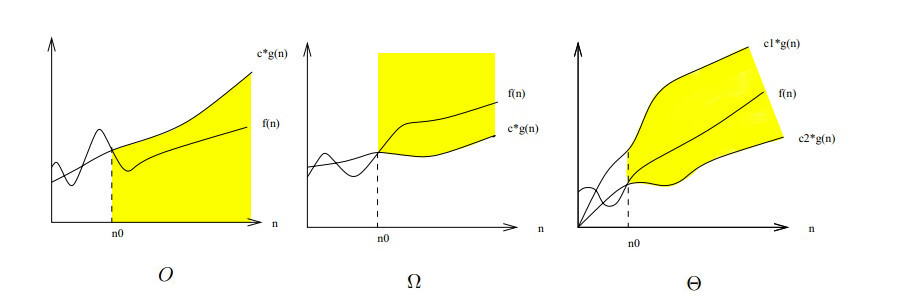
\includegraphics{images/classi_asintotiche.jpg}

Lettura della notazione: \\

$f(n) = \Theta(g(n))$ si legge: $f(n)$ è limitato strettamente da $g(n)$

\paragraph{Proprietà}

\subparagraph{Transitiva}

Se $f(n) = \Theta(g(n))$ e $g(n) = \Theta(h(n))$ allora $f(n) = \Theta(h(n))$ \\
Se $f(n) = O(g(n))$ e $g(n) = O(h(n))$ allora $f(n) = O(h(n))$ \\
Se $f(n) = \Omega(g(n))$ e $g(n) = \Omega(h(n))$ allora $f(n) = \Omega(h(n))$ \\
\\
Se $f(n) = o(g(n))$ e $g(n) = o(h(n))$ allora $f(n) = o(h(n))$ \\
Se $f(n) = \omega(g(n))$ e $g(n) = \omega(h(n))$ allora $f(n) = \omega(h(n))$


\subparagraph{Riflessiva}

$f(n) = \Theta(f(n))$ \\
$f(n) = O(f(n))$ \\
$f(n) = \Omega(f(n))$

\subparagraph{Simmetrica}

$f(n) = \Theta(g(n))$ se e solo se $g(n) = \Theta(f(n))$

\subsection{Limite superiore: Classe O}

O fornisce un limite superiore per la funzione $f(n), \forall n \geq n_0$

\begin{equation}
O(g(n)) = \{f(n) : \exists c,n_0 > 0 \in \mathbb{N}, 0 \leq f(n) \leq c*g(n), \forall n \geq n_0 \}
\end{equation}

\subsection{Limite inferiore: Classe \Omega}

\Omega\, fornisce un limite inferiore per la funzione $f(n), \forall n \geq n_0$

\begin{equation}
O(g(n)) = \{f(n) : \exists c,n_0 > 0 \in \mathbb{N}, 0 \leq c*g(n) \leq f(n), \forall n \geq n_0 \}
\end{equation}

\subsection{Limite stretto: Classe \Theta}

\Theta\, fornisce un limite stretto per la funzione $f(n), \forall n \geq n_0$

\begin{equation}
O(g(n)) = \{f(n) : \exists c_1,c_2,n_0 > 0 \in \mathbb{N}, 0 \leq c_1*g(n) \leq f(n) \leq  c_2*g(n), \forall n \geq n_0 \}
\end{equation}

\subsection{Esercizi sulla notazione asintotica. Le classi o,\omega}}

{{[}CLRS{]} 3.1}

\subsection{Limite inferiore: Classe o}

La classe o è equivalente alla classe O con limite stretto

\begin{equation}
O(g(n)) = \{f(n) : \exists c,n_0 > 0 \in \mathbb{N}, 0 \leq f(n) < c*g(n), \forall n \geq n_0 \}
\end{equation}

\subsection{Limite superiore: Classe \omega}

La classe \omega\, è equivalente alla classe \Omega\, con limite stretto

\begin{equation}
O(g(n)) = \{f(n) : \exists c,n_0 > 0 \in \mathbb{N}, 0 \leq c*g(n) < f(n), \forall n \geq n_0 \}
\end{equation}


\chapter{Analisi delle ricorrenze}

Diversi metodi:

\begin{itemize}
\item Metodo dell'iterazione : il più intuitivo
\item Metodo della sostituzione
\item Teorema master
\item Analisi dell'albero di ricorsione
\item Cambiamenti di variabile
\end{itemize}


\section{Metodo dell'iterazione}


\section{Metodo della sostituzione}


\section{Il teorema fondamentale delle ricorrenze}

{{[}DFI{]} 2.5; {[}CLRS{]} 4.3}


\paragraph{Proprietà 1}
I sottoproblemi al livello i dell'albero della ricorsione hanno dimensione $\frac{n}{b^i}$

\paragraph{Proprietà 2}
Il contributo di un nodo a livello $i$ al tempo di esecuzione (escludendo il tempo speso nelle chiamate ricorsive) è $f\left(\frac{n}{b^i}\right)$

\paragraph{Proprietà 3}
Il numero di livelli nell'albero della ricorsione è $\log_b{n}$

\paragraph{Proprietà 4}
Il numero di nodi al livello $i$ dell'albero della ricorsione è $a^i$

Combinando queste proprietà possiamo riscrivere la relazione di ricorrenza come:

\begin{equation}
T(n) = \sum_{i=0}^{\log_b{n}}{a^if\left(\frac{n}{b^i}\right)}
\end{equation}

La soluzione di questa nuova equazione è data dal teorema fondamentale delle ricorrenze:

\paragraph{Definizione}

Il Teorema Master è un metodo per analizzare algoritmi basati sulla tecnica del dividi et impera in cui

\begin{itemize}
\item un problema di dimensione $n$ viene diviso in $a$ sottoproblemi di dimensione $\frac{b}{n}$
\item dividere in sottoproblemi e combinare le soluzioni richiede tempo $f(n)$
\end{itemize}

\begin{equation}
T(n) = a * T\left(\frac{n}{b}\right) + f(n)
\end{equation}


\begin{teorema}{}{theoexample}

La relazione di ricorrenza
\begin{equation}
T(n) = 
\begin{cases}
1							& \mbox{se } n = 1\\ 
a*T(\frac{n}{b}) + f(n)		& \mbox{se } n > 1
\end{cases}
\end{equation}

ha soluzione

\begin{equation}
T(n) = 
\begin{cases}
\Theta(n^{\log_b{a}})			& \mbox{se } f(n) = O(n^{\log_b{a} - \epsilon}) \mbox{ per } \epsilon > 0\\ 
\Theta(n^{\log_b{a}}*\log{n})			& \mbox{se } f(n) = \Theta(n^{\log_b{a}})  \\ 
\Theta(f(n))			& \mbox{se } f(n) = \Omega(n^{\log_b{a} + \epsilon})  \mbox{ per } \epsilon > 0, \\ 
& a*f(\frac{n}{b}) \leq c*f(n), \\ 
& c < 1, \\
& n \mbox{ sufficientemente grande}
\end{cases}
\end{equation}

\end{teorema}

\subsection{Dimostrazione}

Assunzione: $n = 1, b,b^2,\ldots$ quindi $\frac{n}{b^i}$ sarà sempre intero.

\paragraph{Caso 1}

\begin{equation}
f(n) = O(n^{\log_b{a} - \epsilon}) \mbox{ per } \epsilon > 0
\end{equation}

Riscriviamo in modo più conveniente il generico termine della sommatoria:

$a^if\left(\frac{n}{b^i}\right)=$

$\textcolor{red}{=O\left(a^i\left(\frac{n}{b^i}\right)^{\log_b{a-\epsilon}}\right)}$

$= O\left(\textcolor{red}{n^{\log_b{a-\epsilon}}\left(\frac{a*b^\epsilon}{b^{\log_b{a}}}\right)^i}\right)$

\begin{equation}
= O\left(n^{\log_b{a-\epsilon}}\left(\textcolor{red}{b^\epsilon}\right)^i\right)
\end{equation}

Sostituiamo la complessità all'interno della sommatoria

$T(n) = \sum_{i=0}^{\log_b{n}}{O\left(n^{\log_b{a-\epsilon}}\left(b^\epsilon\right)^i\right)}$

$=O\left(n^{\log_b{a-\epsilon}}\textcolor{red}{\sum_{i=0}^{\log_b{n}}{(b^\epsilon)}^i}\right)$

$=O\left(n^{\log_b{a-\epsilon}}\left(\textcolor{red}{\frac{b^{\epsilon( \log_b{n}+1)}-1}{b^\epsilon-1}}\right)\right)$

$=O\left(n^{\log_b{a-\epsilon}}\left(\frac{\textcolor{red}{b^\epsilon * n^\epsilon} - 1}{b^\epsilon-1}\right)\right)$

$=O\left(n^{\log_b{a-\epsilon}}\textcolor{red}{n^\epsilon}\right)$

\begin{equation}
= O\left(n^{\textcolor{red}{\log_b{a}}}\right)
\end{equation}

Analizzando l’equazione 2.2 e considerando solo i tempi di esecuzione relativi ai nodi sull’ultimo livello dell’albero di ricorsione, otteniamo:

$T(n) \geq a^{\log_b{n}} = \textcolor{red}{n}^{\log_b{\textcolor{red}{a}}}$

Perciò 

$T(n) = \Omega(n^{\log_b{a}})$

Essendo $T(n)$ costretta inferiormente da $\Omega$ e superiormente da $O$, otteniamo che

\begin{equation}
T(n) = \Theta(n^{\log_b{a}})
\end{equation}

\paragraph{Caso 2}

Riscriviamo in modo più conveniente il generico termine della sommatoria:

$a^if\left(\frac{n}{b^i}\right)=$

$\textcolor{red}{=\Theta\left(a^i\left(\frac{n}{b^i}\right)^{\log_b{a}}\right)}$

$=\Theta\left(\textcolor{red}{n^{\log_b{a}} * \left( \frac{a}{b^{\log_b{a}}} \right)^i} \right)$

\begin{equation}
f(n) = \Theta(n^{\log_b{a}})
\end{equation}

Sostituiamo la complessità all'interno della sommatoria:

$T(n) = \sum_{i=0}^{\log_b{n}}{\Theta(n^{\log_b{a}})}$

\begin{equation}
T(n) = \Theta(n^{\log_b{a}}*\log_b{n})
\end{equation}

\paragraph{Caso 3}

\begin{equation}
f(n) = \Omega(n^{\log_b{a} + \epsilon})  \mbox{ per } \epsilon > 0, \\ 
\textcolor{blue}{a*f(\frac{n}{b}) \leq c*f(n), \\ 
c < 1,} \\
n \mbox{ sufficientemente grande}
\end{equation}

Riscriviamo in modo più conveniente il generico termine della sommatoria

$a^i * f\left(\frac{n}{b^i}\right)=$

$=a^{i\textcolor{red}{-1}} \textcolor{red}{* a} * f\left(\textcolor{red}{\frac{\frac{n}{b}^{i-1}}{b}}\right)$

Sotto l’assunzione $\textcolor{blue}{a*f(\frac{n}{b}) \leq c*f(n)}$, risulta facile dimostrare che $a^i * f(n/b^i) \leq c^i * f(n)$ infatti:

$=a^{i-1} * a * f\left(\frac{\frac{n}{b}^{i-1}}{b}\right) \leq a^{i-1} * c * f\left(\frac{n}{b^{i-1}}\right)$

Sostituendo nella sommatoria, la serie geometrica con base $\textcolor{blue}{c < 1}$ e la disuguaglianza appena dimostrata, si può scrivere:


$T(n) = \sum_{i=0}^{\log_b{n}}{a^i * f\left(\frac{n}{b^i}\right)}$

$T(n) \leq f(n) *  \sum_{i=0}^{\infty}{c^i}$

$T(n) = f(n) * \frac{1}{1-c}$

\begin{equation}
T(n) = O(f(n))
\end{equation}

Dalla relazione 2.2, si ricava immediatamente che $T(n) = \Omega(f(n))$, da cui $T(n) = \Theta(f(n))$.

\section{Analisi dell'albero di ricorsione}


\section{Cambiamenti di variabile}



\chapter{Liste}

\section{Rappresentazione di una lista attraverso un vettore (matrice)}

{La lista è doppiamente concatenata, ovvero contiene riferimento sia all'elemento precedente che a quello successivo.}

{La costante NULL viene rappresentata da un indice che non appartiene all'insieme degli indici del vettore (0 in pseudocodice, -1 in $C$)}

\begin{figure}[H]
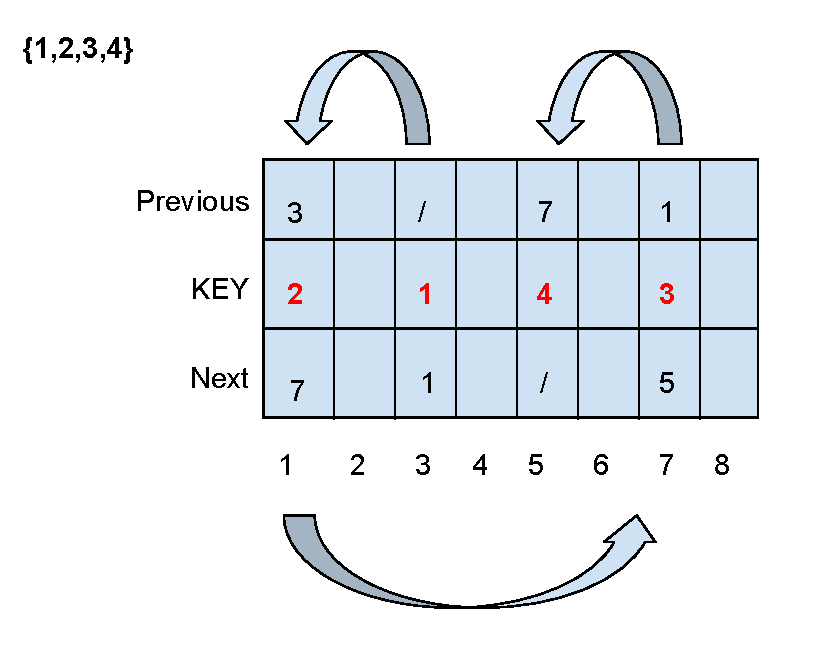
\includegraphics{graphs/lista_matrice.pdf}
\end{figure}

{Analogamente si può creare una lista singolarmente concatenata chiamata FreeList contenente le celle libere (i campi Key e Previous si possono ignorare). Essa verrà utilizzata per l'allocazione di una nuova lista. FreeList è una variabile globale.}

{All'inizio {[}\ldots{}{]} la FreeList contiene TUTTI gli oggetti non allocati.}

{Allocate\_Object()~~~~~~~~~~~~~~~~~~~~~~~~~~~~~~~~}{Complessità $\Theta(1)$}

\lstinputlisting{code/allocate_object.txt}

{\#Inserisce la cella da liberare in testa alla FreeList}

{Free\_Object(x)}{~~~~~~~~~~~~~~~~~~~~~~~~~~~~~~~~Complessità $\Theta(1)$}

\lstinputlisting{code/free_object.txt}


\chapter{Alberi}

{{[}CLRS{]} pp. 977-979}

{L'albero è un tipo particolare di grafo connesso, aciclico e non orientato.}

{Un albero radicato è una coppia $T=(N,A)$}

{$N$ è un insieme finito di nodi fra cui si distingue un nodo $R$, detto `Radice'.}

$A${~è un sottoinsieme del prodotto cartesiano $(NxN)$,è un insieme di coppie di nodi che chiamiamo archi.}

{In un albero, ogni nodo $v$ (eccetto la radice) ha esattamente un genitore che viene chiamato padre $u$, tale che $(u,v) \in A$}

\begin{figure}[H]
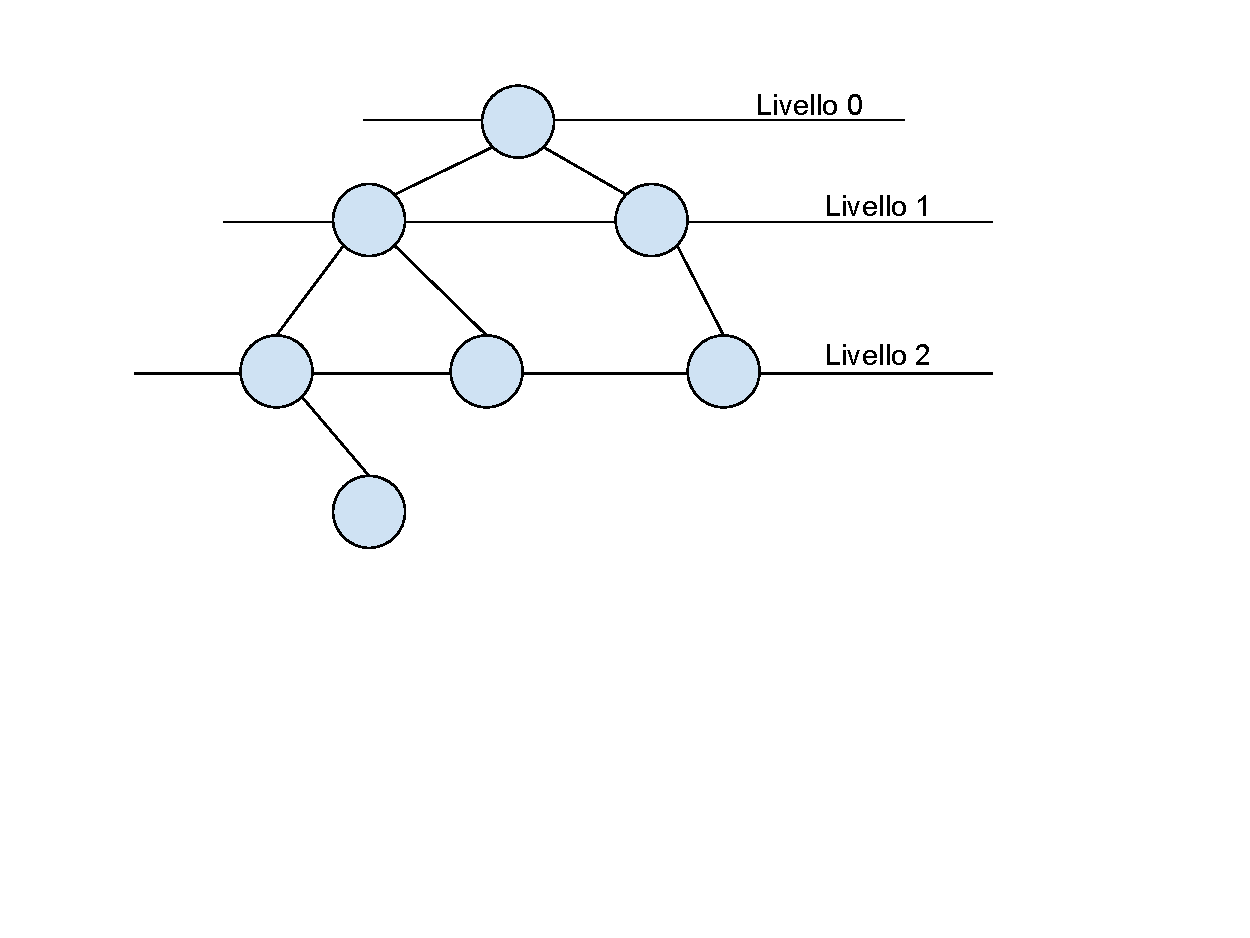
\includegraphics{graphs/alberi_livelli.pdf}
\end{figure}

{Un nodo può avere $0$ o più figli, un figlio è tale se esiste un arco $(u,v) \in A$}

{Il numero dei figli di un nodo si chiama GRADO del nodo.}

{Un nodo senza figli è detto FOGLIA o NODO ESTERNO.}

{Un nodo non foglia è un NODO INTERNO.}

{Se due nodi hanno lo stesso padre, allora sono fratelli.}

{Il cammino da $v$ a $v'$ nell'albero $T$ è una sequenza di nodi $n_0,n_1,\ldots,n_k$ tale che soddisfa queste condizioni:}

$v=n_0$

$v'=n_k$

$(n_{i-i},n_i) \in A\,\forall\,1>i>k$

{La lunghezza di un cammino è il numero di archi nel cammino oppure il numero di nodi diminuito di 1.}

{Sia $x$ un nodo dell'albero radicato $T$ con radice $r$.}

{Qualsiasi nodo $y$ in un cammino, che parte dalla radice $r$ ed arriva ad $x$, è detto ANTENATO di $x$($x$ compreso, è antenato di se stesso).}

{Se $y$ è un antenato di $x$, allora $x$ è DISCENDENTE di $y$}

{NB: Ogni nodo è DISCENDENTE ed ANTENATO di sè stesso.}

{Se $y$ è un antenato di $x$ ed $x$ è diverso da $y$, allora $y$ è un ANTENATO PROPRIO di $x$ ed $x$ è DISCENDENTE PROPRIO di $y$.}

{Il sottoalbero con radice in $x$ è l'albero indotto dai discendenti di $x$}

{La profondità di un nodo $x$ è la lunghezza del cammino dalla radice ad $x$.}

{Un livello di un albero è costituito da tutti i nodi che stanno alla stessa profondità. }

{L'altezza di un nodo $x$ è la lunghezza del più lungo cammino che scende da $x$ alle foglie (qualsiasi foglia) di profondità massima.}

{L'altezza di un albero è l'altezza del nodo radice.}

{L'altezza è la massima profondità di un qualsiasi nodo dell'albero.}

\subsection{Alberi binari}

{Gli alberi binari sono definiti in modo ricorsivo:}

\begin{itemize}
\tightlist
\item
  {Un albero vuoto è binario}
\item
  {Un albero costituito da un nodo (radice) ,}
\end{itemize}

{~~~~~~~~~~~~~~~~da un albero binario detto sottoalbero sinistro della
radice,}

{~~~~~~~~~~~~~~~~e da un'altro albero binario detto sottoalbero destro
della radice}

{~~~~~~~~~~~~~~~~è detto un albero binario.}

\subsection{Albero k-ario}

{E' un albero in cui i figli si un nodo sono etichettati con interi positivi distinti e le etichette maggiori di $K$ sono assenti = ogni nodo può avere al più $K$ figli.}

{Un albero K-ario completo è tale quando tutte le foglie hanno la stessa profondità e tutti i nodi interni hanno grado $K$}

\paragraph{ALGORITMO}

{Trovare l'algoritmo per determinare la completezza di un albero}

{Dimostro per induzione che le foglie sono $K^h$}


{$h=0$ (caso base): $K^0=1$, OK}

{Assumiamo che per un albero di altezza $h$ sia vero che $n=K^h$}

{Lo dimostro per $h+1$}

{Il numero di nodi di profondità $h$ è $K^h$ per ipotesi}

{Il numero di nodi di profondità $h+1$ è $K^h*K=K^{h+1}$, OK}

\paragraph{ALGORITMO}

{Trovare il numero di foglie e il numero di nodi interni di un albero k-ario completo di altezza $h$}

{$\sum_{\varphi=0}^{h-1}{K^{\varphi}}$ è una sommatoria GEOMETRICA, si semplifica in $\frac{K^{h-1+1}-1}{K-1}$ con $k\neq 1$, quindi $\frac{K^h-1}{K-1}$}

{Altezza di un albero k-ario completo con $n$ nodi:}

$n=K^h \rightarrow log_k(n) = log_k(K^h) \rightarrow log_k(n) = h$

\paragraph{Proprietà}

{Dimostrare per induzione che in un albero BINARIO completo non nullo avente $n$ nodi, il numero di foglie è $\frac{n+1}{2}$}

\subsubsection{Tipo di dato ALBERO}

{Struttura:}

{Insieme di nodi}

{Insieme di archi}


{Le operazioni del tipo ALBERO:}


{~~~~~~~~newTree() → T~~~~~~~~~~~~~~~~Nuovo albero T}

{~~~~~~~~numNodi(T) → int~~~~~~~~~~~~~~~~Numero di nodi presenti in T}

{~~~~~~~~grado(T,N) → int~~~~~~~~~~~~~~~~Numero di figli di N, N
appartenente a T}

{~~~~~~~~padre(T,N) → int~~~~~~~~~~~~~~~~Nodo padre, null se N è radice,
~N appartenente a T}

{~~~~~~~~figli(T,N) → int{[}{]}~~~~~~~~~~~~~~~~Lista contenente i figli
del nodo N, N appartenente a T}

{}

\subsection{Rappresentazione di alberi tramite array}

\subsubsection{Utilizzo del vettore padri}

{Sia $T=(N,A), N = \{n_1,n_2,\ldots,n_n\}$}

{Costruisco un vettore di dimensione $n$, le cui celle contengono copie di $(i,u)$. Con $i$ indichiamo l'informazione del nodo e con $u$ indichiamo il nodo padre (indice).}

$\forall v \in [1,n]$

{p{[}v{]} → info = contenuto}

{p{[}v{]} → padre = indice del padre,$(u,v) \in A(archi)$, se $v$ è radice il padre è $NULL/-1/0$}

{Spazio per memorizzare $n=\Theta(n)$}

\paragraph{Implementazioni}

{Padre - Complessità $\Theta(1)$}

\lstinputlisting{code/tree_vecp_padre.txt}

{Figli - Complessità $\Theta(n)$}

\lstinputlisting{code/tree_vecp_figli.txt}

\subsubsection{Utilizzo del vettore posizionale}

{L'albero deve essere completo e con $k \geq 2$. La ricerca è ottimizzata rispetto all'albero dei padri. Ogni nodo ha una posizione prestabilita.}

{Utilizzo un vettore posizionale $P$ di dimensione $n$ tale che }

\begin{enumerate}
\tightlist
\item
  {0 è la posizione della radice}
\item
  {l'i-esimo figlio di un certo nodo $v$ è in posizione $kv+i+1$, con $0\leq i < K-1$}
\end{enumerate}

{un nodo $f$ è foglia se non ha figli, quindi se $kv+1>n$}

{Il padre del nodo $f$ è in posizione $\floor{\frac{f-1}{k}}$ (parte intera inferiore) e i figli si trovano tra $kv+1$ e $kv+1+i-1$.

\paragraph{Implementazioni}

{Padre - Complessità $\Theta(1)$}

\lstinputlisting{code/tree_vec_padre.txt}

{Figli - Complessità $\Theta(k)$, con $k$ = grado di $v$}

\lstinputlisting{code/tree_vec_figli.txt}

\subsubsection{Utilizzo di strutture collegate}

\paragraph{Parent + Childs}

{}

{Ogni nodo è un record con i seguenti campi:}

{~~~~~~~~k : informazione}

{~~~~~~~~p : puntatore al padre}



{~~~~~~~~Se il numero di figli è noto}

{}

{~~~~~~~~~~~~~~~~left : puntatore al figlio sinistro}

{~~~~~~~~~~~~~~~~right : puntatore al figlio destro}

{}

{Altrimenti si utilizza una lista di puntatori ai propri figli}

{c {[}{]} : lista di puntatori ai figli~~~~~~~~}

{Se ogni nodo ha grado al più $k$, è possibile mantenere in ogni nodo un puntatore a ciascuno dei possibili $k$ figli}

{Spazio necessario: $\Theta(nk)$, se $k$ costante allora $\Theta(n)$}

\paragraph{Implementazioni:}

{Padre - Complessità $O(1)$}

\lstinputlisting{code/tree_pc_padre.txt}

{Figli - Complessità $O(k)$, con $k$ = grado di $v$ }

{Con $k$ non noto si utilizza un ciclo che scorre c{[}{]}}

\lstinputlisting{code/tree_pc_figli.txt}

\paragraph{Parent + Left child + Right sibling}

{Ogni nodo è un record con i seguenti campi:}

{~~~~~~~~k : informazione}

{~~~~~~~~p : puntatore al padre}

{~~~~~~~~left\_child : puntatore al figlio sinistro}

{~~~~~~~~right\_sibling : puntatore al fratello immediatamente a destra}

\paragraph{Implementazioni}

{Padre - Complessità $\Theta(1)$}

\lstinputlisting{code/tree_plcrs_padre.txt}

{Figli - Complessità $\Theta(k)$ con $k$ = grado di $v$}

\lstinputlisting{code/tree_plcrs_figli.txt}

\subsection{Algoritmi di visita degli Alberi}

{{[}DFI{]} pp. 77-80}

\subsubsection{Visita generica}

\lstinputlisting{code/visita_generica.txt}

{Dimostrare che ha costo LINEARE}\textsuperscript{\protect\hyperlink{cmnt2}{{[}b{]}}}

\paragraph{Teorema}

{L'algoritmo di visita, applicato alla radice di un albero con $m$ nodi, termina in $O(m)$ iterazioni. Lo spazio usato è $O(n)$}

\paragraph{Dimostrazione}

{Hp: L'inserimento e la cancellazione da $S$ sono effettuati in tempo costante}

{Ogni nodo verrà inserito ed estratto dall'insieme $s$ una sola volta, perchè in un albero non si può tornare ad un nodo a partire dai suoi figli.}

{Quindi le iterazioni del ciclo while saranno al più $O(n)$}

{Poiché ogno nodo compare al più una volta in $S$, lo spazio richiesto non è più alto di $O(n)$}

\subsubsection{Visita DFS - Depth first search - Ricerca in profondità}

{Seguiamo tutti i figli sinistri, andando in profondità fino a che non si raggiunge la prima foglia sinistra. Solo quando il sottoalbero sx è stato completamente visitato, si passa ~a visitare il sottoalbero dx}

\lstinputlisting{code/dfs_visit.txt}

\subsubsection{Visita BFS - Breadth first search - Ricerca in ampiezza}


\chapter{Heap}

{Heap: albero quasi completo con tutti i nodi dell'ultimo livello a sinistra}

{MaxHeap: La radice ha valore maggiore o uguale a quello dei figli}

{MinHeap: La radice ha valore minore o uguale a quello dei figli}


\begin{lemma}{Lemma 2}{theoexample}
Nell'array che rappresenta un heap di $n$ elementi, le foglie sono i nodi con indici che vanno alle posizioni

$\frac{n}{2}+1,\frac{n}{2}+2,\ldots,n$

\end{lemma}

\paragraph{Esempio:}

\begin{tikzpicture}[>=stealth, every node/.style={circle, draw, minimum size=0.75cm}]
\graph [tree layout, grow=down, fresh nodes, level distance=0.5in, sibling distance=0.5in]
    {
        16 -> { 
          15 -> { 14 -> { 2, 8 }, 7 -> {1} },
          10 -> { 9, 3 }
        } 
    };
\end{tikzpicture}

\begin{tabular}{|c|c|c|c|c|c|c|c|c|c|c|}
\hline
Elemento & 16 & 15 & 10 & 14 & 7 & 9 & 3 & 2 & 8 & 1 \\
\hline
Posizione & 1 & 2 & 3 & 4 & 5 & 6 & 7 & 8 & 9 & 10 \\
\hline
 &  &  &  &  & $\frac{n}{2}$ & $\frac{n}{2}+1$ & $\frac{n}{2}+2$ & $\frac{n}{2}+3$ & $\frac{n}{2}+4$ & $n$ \\
\hline
\end{tabular}

\subsubsection{Lemma 3}

{Altezza di un nodo: cammino più lungo verso una foglia}

{Il teorema definisce la numerosità di nodi con una certa altezza:}

{Ci sono al massimo $\frac{n}{2^{h+1}}$ nodi di altezza $h$ in
un qualsiasi heap di $n$ elementi}

\subsubsection{Max\_heapify}}}

{L'operazione max\_heapify permette di mantenere le proprietà di maxheap}

{Precondizioni:}

{Gli alberi binari con radice in left(i) e right(i) sono maxheap}

{Postcondizioni:}

{~~~~~~~~L'albero radicato in $i$ è un maxheap}

\lstinputlisting{code/max_heapify.txt}

{Tempo di esecuzione : $O(h)$ dove $h$ è l'altezza del nodi i poichè l'heap ha altezza $log(n)$ (LEMMA 2)}

\subsection{Dato un vettore disordinato, costruire un heap}

\lstinputlisting{code/build_maxheap.txt}

{Invariante: ogni nodo in posizione $i+1,\ldots,n$ è radice di un maxheap, con n = MANCA}

{Sembrerebbe complessa $O(\frac{n}{2}\,log(n)) = O(n\,log(n))$ ma max\_heapify lavora principalmente su foglie, quindi la complessità è lineare $O(n)$.}

\begin{equation}
\sum_{h=0}^{log(n)}{\floor*{\frac{h}{2^{h-1}}}*O(h)} = O(n*\sum_{h=0}^{log(n)}{\floor*{\frac{h}{2^h}})}
\end{equation}

{L'ultima sommatoria è la serie nota}

\begin{equation}
\sum_{h=0}^{+\infty}{h*x^h} = \frac{x}{{(1-x)}^2}
\end{equation}

{Con $x=\frac{1}{2}$:}

\begin{equation}
\sum_{h=0}^{+\infty}{h*x^h} = \frac{\frac{1}{2}}{{(1-\frac{1}{2})}^2} = 2
\end{equation}

{Quindi}

\begin{equation}
O(n*\sum_{h=0}^{log(n)}{\floor*{\frac{h}{2^h}}}) = O(2n) = O(n)
\end{equation}

\subsection{Heapsort}

\lstinputlisting{code/heapsort.txt}

{INV = Il sottoarray che va dalla posizione $1$ alla posizione $i$ è un maxheap che contiene gli elementi più piccoli del intero vettore di partenza, mentre $A[a+1,\ldots,n]$ contiene gli $n-1$ elementi più grandi di $A[1..n]$ ordinati}{.}

\begin{teorema}{ }{theoexample}
L'algoritmo HeapSort ordina in loco $n$ elementi eseguendo nel peggiore dei casi $O(nlog(n))$ confronti in quanto algoritmo basato sui confronti.
\end{teorema}

\subsection{Code di priorità}

{{[}CLRS{]} pp. 135-140}

{Struttura dati che serve a mantenere un insieme dinamico i cui elementi ( aggiungibili e rimovibili ) hanno un valore associato detto chiave o peso.}

{Esistono due tipi di code di priorità:}

\begin{itemize}
\tightlist
\item
  {MaxPriorità (Si utilizza la struttura MaxHeap)}
\item
  {MinPriorità (Si utilizza la struttura MinHeap)}
\end{itemize}

{Le operazioni delle code di priorità massima/minima sono:}

{Insert( Coda s , Elemento X) : Inserisce l'elemento $X$ in $S$}

{Maximum( Coda s ): Restituisce l'elemento di $S$ con la chiave maggiore senza rimuoverlo}

{Minimum( Coda s) : Restituisce l'elemento di $S$ con la chiave minore senza rimuoverlo}

{Extract\_max( Coda s) : Elimina e restituisce l'elemento di $S$ con la chiave maggiore}

{Extract\_min( Coda s) : Elimina e restituisce l'elemento di $S$ con la chiave minore}

{Increase\_key( Coda s, Elemento x, Chiave k) : Incrementa il valore della chiave di $X$ al nuovo valore $K$. Si suppone che $K$ sia maggiore o uguale al valore corrente della chiave di $X$, $K \geq chiave(X)$}

{Decrease\_key( Coda s, Elemento x, Chiave k) : Decrementa il valore della chiave di $X$ al nuovo valore $K$. Si suppone che $K$ sia minore o uguale al valore corrente della chiave di $X$, $K \leq chiave(X)$}

\begin{center}\rule{0.5\linewidth}{\linethickness}\end{center}

\subsection{Implementazione di code di massima priorità tramite Heap}

\lstinputlisting{code/heap_maximum.txt}

{Complessità di Heap Maximum : $O(1)$}

\lstinputlisting{code/heap_extract_max.txt}

{Complessità di Heap Extract Max : $O(log(n))$}

\lstinputlisting{code/heap_increase_key.txt}

{Complessità di Heap Increase Key : $O(log(n))$}

{Invariante del while: L'array $A[i,\ldots,A.heapSize]$ soddisfa le proprietà di maxHeap tranne una possibile violazione: A{[}i{]} potrebbe essere più grande di A{[}parent(i){]}}

{Con un Heap di n elementi, la complessità è $O(log(n))$ in quanto il cammino dal nodo fino alla radice ha lunghezza }$O(log(n))$

\lstinputlisting{code/heap_insert.txt}

{Complessità di Heap\_Insert : }$O(log(n))$

{La ricerca su una cosa di priorità, nel caso peggiore, ha costo }$O(n)$

{Premessa : $1 \leq i \leq A.heapSize$}

\lstinputlisting{code/heap_delete.txt}

{Complessità di Heap Delete : }$O(log(n))$

\paragraph{Esercizio 1}

{Scrivere una funzione che determini se un albero è quasi completo. Gli output devono essere 1 se l'albero è quasi completo o 0 se non lo è. }{L'albero è rappresentato con notazione left e right.}

{Note: notiamo che non è sufficiente sapere se un albero è quasi completo o meno, necessitiamo anche di un valore per rappresentare l'albero completo.}

{Gli output saranno quindi: 0 - albero completo, 1 - albero quasi completo, 2 - albero non quasi completo.}

\lstinputlisting{code/is_quasi_completo.txt}

\lstinputlisting{code/is_quasi_completo_aux.txt}

{Complessità di is\_quasi\_completo : $O(n)$}

$T(n) = T(k) + T(n-k-1) + c = O(n)$

\paragraph{Esercizio 2}

{Siano dati due alberi binari completi di radice $r$ ed $s$ aventi la stessa altezza $h$ e dimensione totale (somma dei nodi dei due alberi) $n$. Le chiavi memorizzate nei nodi soddisfano la proprietà di maxheap. Si vuole creare un unico albero quasi completo maxheap, fusione dei due alberi, con altezza $h+1$ e dimensione $n$.}

{Le seguenti soluzioni vengono accettate:}

\begin{enumerate}
\tightlist
\item
  {Soluzione di costo e tempo $\Theta(n)$ e in spazio aggiuntivo $\Theta(n)$}
\item
  {Soluzione (più elegante) di costo e tempo $O(log(n))$ e spazio aggiuntivo costante}
\end{enumerate}

{Soluzione :}

\begin{enumerate}
\tightlist
\item
  {Soluzione di costo e tempo $\Theta(n)$ e in spazio aggiuntivo $\Theta(n)$}
\end{enumerate}

{~~~~~~~~~~~~~~~~~~~~~~~~Vettore di n elementi v. (spazio aggiuntivo $\Theta(n)$)}

{~~~~~~~~~~~~~~~~~~~~~~~~Carichiamo il vettore con i valori di $r$ ed $s$. $\Theta(n)$}

{~~~~~~~~~~~~~~~~~~~~~~~~Applichiamo build\_maxheap all'intero vettore $v$. $\Theta(n)$}

{~~~~~~~~~~~~~~~~~~~~~~~~Creo l'albero corrispondente. $\Theta(n)$}

\begin{enumerate}
\setcounter{enumi}{1}
\tightlist
\item
  {Soluzione di costo e tempo $O(log(n))$ e spazio aggiuntivo costante}
\end{enumerate}

{Non possiamo fare altro che modificare le strutture a nostra disposizione, non usiamo strutture ausiliarie.}

{Prendo come radice il nodo foglia $x$ più a destra dell'albero $s$. $\Theta(log(n))$}

{Assegno $x.left$ ad $s$ e $x.right$ ad $r$.}

{Applico la max\_heapify al nuovo nodo radice x. $\Theta(log(n))$}


\chapter{Ordinamenti}

\section{Limite inferiore per l'ordinamento per confronti}

{{[}CLRS{]} pp. 157-159}

{Fino ad ora abbiamo visto i seguenti algoritmi di ordinamento, tutti basati sul confronto.}

\begin{tabular}{|c|c|}
\hline
Algoritmo & Complessità \\
\hline
MergeSort & $\Theta(n\,log(n)))$ \\
\hline
QuickSort & Caso medio : $\Theta(n\,log(n)))$, caso pessimo : $\Theta(n^2)$ \\
\hline
HeapSort & $\Theta(n\,log(n)))$ \\
\hline
InsertionSort & $\Theta(n^2)$ \\
\hline
\end{tabular}

{Ci domandiamo, è possibile infrangere il limite inferiore di $\Theta(n\,log(n))$? Dimostreremo che NON è possibile farlo con algoritmi basati sul confronto.}

{Analizziamo il limite inferiore degli algoritmi basati sul confronto:}

{$\Omega(n)$ è il limite banale, in quanto devo analizzare n elementi. Questo limite è tuttavia irrealistico e insensato.}

{Tutti gli algoritmi basati sul confronto hanno come limite inferiore $\Omega(n\,log(n))$. Per dimostrarlo facciamo uso degli alberi di decisione.}

{Un albero di decisione è un'astrazione di un qualsiasi algoritmo di ordinamento basato sui confronti.}

\subsection{Esempio: Ordina 3 elementi}

{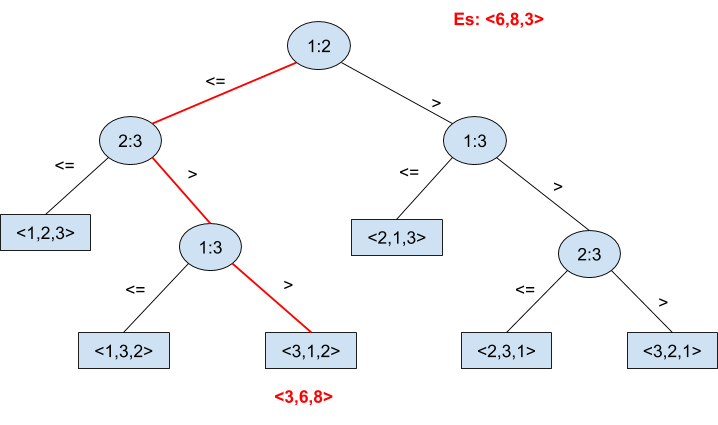
\includegraphics{images/image531.png}}

{Questa struttura assomiglia all'InsertionSort}\textsuperscript{\protect\hyperlink{cmnt15}{{[}o{]}}}

{Per un input $A = <A_1,\ldots,A_n>$ di dimensione $n$, ogni nodo interno è etichettato da una coppia $i:j$ dove $i,j$ sono indici dell'insieme da ordinare.}

\begin{itemize}
\tightlist
\item
  {$i:j$ significa confrontare $A_i$ con $A_j$}
\item
  {il sottoalbero sinistro dà i successivi confronti se $A_i \leq A_j$}
\item
  {il sottoalbero destro dà i successivi confronti se $A_i > A_j$}
\item
  {ogni foglia fornisce una permutazione dell'input tale che se io vado a prendere gli elementi dell'input, ordinati a seconda della permutazione, ottengo l'insieme ordinato in ordine crescente}
\end{itemize}

{Dato un qualsiasi algoritmo di ordinamento basato sul confronto, è possibile costruirmi gli alberi di decisione.}

\begin{itemize}
\tightlist
\item
  {Ogni valore di n è associato ad un proprio albero di decisione.}
\item
  {L'albero modella tutte le tracce possibile di esecuzione.}
\item
  {Il tempo di esecuzione (cioè il numero di confronti necessari) è la lunghezza di un cammino sull'albero.}
\item
  {Il tempo di esecuzione nel caso peggiore è il più lungo cammino dell'albero, ovvero l'altezza dell'albero.}
\end{itemize}

{Mi basta quindi trovare la dimensione dell'albero di decisione per
determinare il tempo di esecuzione.}

\subsection{Quanto è grande un albero di decisione?}

\subsubsection{Quante foglie contiene?}

{L'albero ha come minimo $n!$ foglie poichè, per essere corretto, ogni permutazione deve comparire almeno una volta.}

\paragraph{Lemma 2}

{Un albero binario di altezza h ha al più $2^h$ foglie.}

{Dimostrazione per induzione:}

\begin{itemize}
\tightlist
\item
  {Se $h=0$ abbiamo un albero costituito da un solo nodo radice che è l'unica foglia. Ovviamente con $h=0$, $1 \leq 2^h$ è verificata, infatti $1\leq 2^0$.}
\item
  {Assumiamo vera la proprietà per alberi binari di altezza $k<h$ e lo dimostro per $h$. Sia $r$ la radice dell'albero $t$. }
\end{itemize}

\begin{itemize}
\tightlist
\item
  {Se $t$ ha un solo figlio allora il numero di foglie di $t$ è uguale a quello del figlio che ha altezza $h-1$. }{Per ipotesi induttiva}{: Il numero delle foglie del sottoalbero figlio è minore di $2^{h-1}$, che è minore di $2^h$.}
\item
  {Se sono presenti entrambi il figlio sx e il figlio dx, allora il numero delle foglie è dato dalla somma delle foglie dei due sottoalberi. Siano $h_L,h_R$ le altezze dei due figli. Entrambe sono minori di $h$.}
\end{itemize}

\begin{equation}
f=f_L+f_R = 2^{h_L} + 2^{h_R} \leq 2 * 2^{max(h_L,h_R)}
\end{equation}

{$f \leq 2^{1+max(h_L,h_R)}$ ma $1+max(h_L,h_R) = h$, quindi $f \leq 2^h$}

{Quindi il numero delle foglie è compreso tra $n!$ e $2^h$.}

\paragraph{Teorema:}

{Qualsiasi algoritmo di ordinamento per confronti richiede almeno $\Omega(n\,log(n))$ confronti nel caso peggiore.}

{Dimostrazione:}

{Bisogna determinare l'altezza di un albero di decisione, dove ogni permutazione appare come foglia. Si consideri un albero di decisione di altezza $h$ con $l$ foglie che corrisponde ad un ordinamento per confronti di $n$ elementi. }

{Allora $n! \leq l \leq 2^h$ (per Lemma 2)}

{Passando al logaritmo, $h \geq log(n!)$}

{Utilizziamo l'approssimazione di \href{https://www.google.com/url?q=https://it.wikipedia.org/wiki/Approssimazione_di_Stirling\&sa=D\&ust=1523379128517000}{Stirling} per approssimare $n!$:}

\begin{equation}
n! \simeq \sqrt{2\pi n }* {(\frac{n}{e})}^n
\end{equation}

{Per n sufficientemente grande, considero solo il termine più grande}

$h \geq log({(\frac{n}{e})}^n)$

{Per proprietà dei logaritmi}

$h \geq n*log(\frac{n}{e})$

{$h \geq n*(log(n) - log(e))$ , il secondo algoritmo è costante}

$n \geq n * log(n)$

{Non ci può essere quindi un algoritmo basato sui confronti minore di $n * log(n)$}

\paragraph{Corollario:}

{Gli algoritmi HeapSort e MergeSort sono algoritmi di ordinamento per confronti asintoticamente ottimali.}

{Dimostrazione:}

{I limiti superiori dei sue algoritmi sono $O(n\,log(n))$ nei tempi di esecuzione corrispondono al limite inferiore $\Omega(n\,log(n))$ nel caso peggiore dato dal teorema.}

{Se elimino il modello basato sui confronti, posso battere il limite inferiore di $\Omega(n\,log(n))$? SI.}



\subsection{Algoritmi di ordinamento privi di confronti}

\subsubsection{CountingSort}

{{[}CLRS{]} pp. 159-161}

{Assunzione:}

{~~~~~~~~I numeri da ordinare sono interi in un intervallo che va da 0 a $k$, per qualche $k$ prefissato}

{Input:}

{$A=[0,\ldots,n]$ dove $A[j] \in [0,\ldots,k]$, $n,k$ sono parametri}

{Output:}

{$B=[0,\ldots,n]$ ordinato, permutazione di A}

{Utilizzo una memoria ausiliaria $C$, costituita da $k+1$ elementi, $C=[0,\ldots,n]$}

{Codice:}

\lstinputlisting{code/counting_sort.txt}

{Complessità di CountingSort : $\Theta(n+k)$}

{Di solito il CountingSort quando $k$ è limitato superiormente da n, $k=O(n)$. Allora il tempo di esecuzione risulta $\Theta(n)$. Il tempo di esecuzione di questo algoritmo è dato da
$\Theta(n+k)$. Il CountingSort di solito è utilizzato quando $k$ è limitato superiormente da $n$ in $k=O(n)$. Allora, il tempo di esecuzione risulta essere $O(n)$.}

{Il CountingSort è un algoritmo stabile, caratteristica molto importante.}

{Analisi:}

{~~~~~~~~All'uscita dal secondo ciclo: $C[i] = \abs{\{x \in \{1\ldots n\}\,|\,A[x] = i\}}$}

{~~~~~~~~All'uscita dal terzo giro: $C[i] = \abs{\{x \in \{1\ldots n\}\,|\,A[x] \leq i\}}$}


\subsubsection{RadixSort}

{{[}CLRS{]} pp. 162-164}

{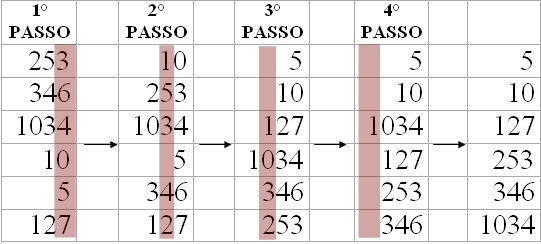
\includegraphics{images/image540.png}}

{L'algoritmo di ordinamento scelto deve essere stabili e rispettare l'ordine.}

\lstinputlisting{code/radix_sort.txt}

{Dimostriamo la correttezza dell'algoritmo tramite induzione sulla colonna da ordinare:}

{Caso base (i=1)}

{~~~~~~~~Ordino l'unica colonna}

{Assumo che le cifre delle colonne che vanno da $1$ a $i-1$ siano ordinate}

{Dimostro che un algoritmo stabile sulla colonna $i$, lascia le colonne da $1$ a $i$ ordinate:}

{Se due cifre in posizione $i$}

\begin{itemize}
\tightlist
\item
  {sono uguali: per stabilità, rimangono nello stesso ordine e, per ipotesi induttiva, sono ordinate.}
\item
  {sono diverse: l'algoritmo di ordinamento sulle colonna $i$ le ordina e le mette in posizione corretta.}
\end{itemize}

{Complessità: $\Theta(d*(k+n))$}

{Teorema: }

{Dati $n$ numeri di $d$ cifre, dove ogni cifra può avere fino a $k$ valori possibili}\textsuperscript{\protect\hyperlink{cmnt16}{{[}p{]}}}{, la procedura ordina correttamente i numeri nel tempo di $\Theta(d*(k+n))$ se l'algoritmo stabile utilizzato dalla procedura impiega un tempo $\Theta(k+n)$}

{Dimostrazione:}

{Per ogni iterazione, il costo risulta essere $\Theta(k+n)$}

{Le iterazioni sono $d$, per un totale di $\Theta(d*(k+n))$}

{Osservazioni:}

{~~~~~~~~Se $k=O(n)$ il tempo di esecuzione è $\Theta(d*n)$}

{Inoltre, se $d$ è costante, la complessità è $\Theta(n)$}

\paragraph{Come ripartire le chiavi in cifre?}

\begin{itemize}
\tightlist
\item
  {Usiamo il CountingSort su ciascuna cifra $\Theta(k+n)$}
\item
  {Siano }$n${~interi, ognuno costituito da $b$ bits}
\item
  {Divido ogni intero in $\ceil*{\frac{b}{r}}$ ``cifre'', ognuna di $r$ bits. La cifra appartiene a $[0,\ldots,2^r-1]$, $k=2^r$}
\end{itemize}

{Esempio: Parola di 32 bits}

{La suddivido in cifre, ciascuna di 8 bits}

$b=32, r=8, d=4$ (4 cifre)

$\Theta(\frac{b}{r}*(n+k))$

$\Theta(\frac{b}{r}*(n+2^r)) = \Theta(\frac{b}{r}*n + \frac{b}{r}*2^r)$

{Cerco di minimizzare la complessità ponendo $r$ grande, $\frac{b}{r}*n$ risulta diminuito, ma $\frac{b}{r}*2^r$ è cresciuto esponenzialmente. Scelgo $r$ piccolo, altrimenti $2^r$ domina su $n$.}

{Scegliamo $r$ essere il massimo valore tale che $n$ risulti essere $n\geq 2^r$, quindi $r=log(n)$.}

{Sostituendo:}

{$\Theta(\frac{b}{log(n)}*(n+2^{log(n)}))$, essendo $2^{log(n)} = n$, abbiamo $\Theta(\frac{b}{log(n)}*n)$}

{I numeri variano nell'intervallo $[0,\ldots,2^b-1]$. Se fisso $b=c*log(n)$, allora l'intervallo diventa $[0,\ldots,n^c-1]$.}

{Allora il tempo è uguale a $\Theta(c*n)$, se $c$ è costante, allora il tempo è $\Theta(n)$.}

{Ho ampliato la grandezza dell'intervallo su cui posso applicare l'algoritmo.}



\chapter{Tabelle hash}

{{[}CLRS{]} pp. 209-211}

{Le tabelle hash sono una possibile implementazione dei dizionari,insiemi dinamici con inserimento, cancellazione e ricerca dove ogni elemento è associato ad una chiave.}

{I dizionari possono essere implementati nei seguenti modi:}

\begin{itemize}
\tightlist
\item
  {Liste: $O(n)$}
\item
	{Alberi binari}

\begin{itemize}
\tightlist
\item
  	{Non bilanciati: $O(n)$}
\item
  	{Bilanciati: $O(log(n))$}
\end{itemize}

\item
  	{Tabelle hash}

\begin{itemize}
\tightlist
\item
	{Tempo medio: $\Theta(1)$ (Motivo principale per l'utilizzo delle tabelle hash)}
\item
	{Caso peggiore: $\Theta(n)$}
\end{itemize}

\end{itemize}

{Vogliamo fornire un'applicazione che ha bisogno di un insieme dinamico (insert/delete/search). Ogni elemento ha una chiave estratta da un universo $\mathbb{U}$ con $\abs{\mathbb{U}} = \{0,\ldots,w-1\}$, dove $w$ non è troppo grande. Nessun elemento ha la stessa chiave (elementi distinti). }

{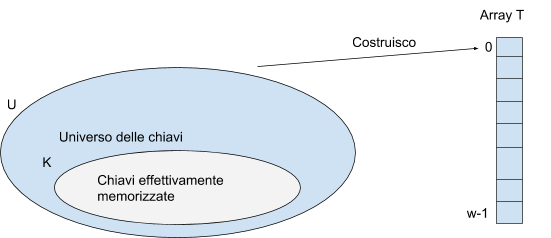
\includegraphics{images/image521.png}}

{Mi costruisco una tabella ad accesso diretto. Si può utilizzare un array $[0,\ldots,w-1]$ dove}

\begin{itemize}
\tightlist
\item
  {ogni posizione (o cella) corrisponde ad una chiave di $\mathbb{U}$}
\item
  {Se c'è un elemento $x$ con chiave $k$, allora nella posizione $T(k)$ è contenuto un puntatore a $x$}
\item
  {Altrimenti, se l'insieme non contiene l'elemento, $T(k) = NULL$}
\end{itemize}

\begin{equation}
T(k) =
\begin{cases}
x & \mbox{se } x.key=k, x\in K \\
NULL & \mbox{altrimenti}
\end{cases}
\end{equation}

{Direct\_Access\_Search : }$O(1)$

\lstinputlisting{code/direct_access_search.txt}

{Direct\_Access\_Insert : $O(1)$}

\lstinputlisting{code/direct_access_insert.txt}

{Direct\_Access\_Delete : $O(1)$}

\lstinputlisting{code/direct_access_delete.txt}

{Potrebbe essere uno spreco se $\abs{K} \ll \abs{\mathbb{U}}$ (Molto minore)}

{Pregi:}

{Operazioni eseguibili in tempo costante}

{Difetti:}

{Lo spazio utilizzato è proporzionale a $w$ e non al numero $n$ di elementi. Di conseguenza si può avere un importante spreco di memoria.}

{Per ovviare al problema dello spreco di memoria si utilizzano le tabelle hash.}

{Richieste:}

\begin{enumerate}
\tightlist
\item
  {Vogliamo ridurre lo spazio per la tabella ad $\Theta(\abs{K})$, ovvero il numero di chiavi
  effettivamente utilizzate}
\item
  {Le operazioni siano con costo medio $\Theta(1)$, ma non nel caso pessimo}
\end{enumerate}

{Idea:}

{Invece di memorizzazione un elemento con chiave o nella cella $k$, si usa una funzione $h$, detta funzione hash, e si memorizza l'elemento nella cella $h(k)$}


{$h:\mathbb{U}\rightarrow\{0,1,\ldots,m-1\}$, dove $m$ della tabella hash è generalmente molto più piccola della dimensione dello spazio di tutte le chiavi.}

{Problema: }

{Se $m < \abs{\mathbb{U}}$, due valori possono essere mappati nella stessa cella, ciò è chiamato collisione. }

{Le tabelle hash possono soffrire del problema delle collisioni: quando un elemento da inserire è mappato, tramite $h$, in una cella già occupata, si verifica una collisione.}

$k_1 \neq k_2 \in \mathbb{U}, h(k_1) = h(k_2)$

{Se $\abs{K} > m$, ho la certezza di imbattermi in collisioni.}

{Cerchiamo quindi strategie per gestire le collisioni, ne analizzeremo due:}

\begin{enumerate}
\tightlist
\item
  {Metodo di concatenamento (liste di collisione (o di trabocco))}
\item
  {Indirizzamento aperto}
\end{enumerate}

\subsection{Risoluzione delle collisioni tramite metodo di concatenamento}

{Si mettono tutti gli elementi che sono associati alla stessa cella in una lista concatenata.}

{La cella $j$ contiene un puntatore alla testa di una lista di tutti gli elementi memorizzati che sono mappati in $j$. Se non ci sono elementi, la cella $j$ conterrà $NULL$.}

\subsubsection{Implementazioni}

{Andiamo ad analizzare l'hashing con concatenamento.}

\lstinputlisting{code/chained_hash_insert.txt}

{Tempo di esecuzione: $\Theta(1)$ se $h$ impiega tempo costante $\Theta(1)$ e l'elemento non è presente nella lista}

\lstinputlisting{code/chained_hash_search.txt}

{Tempo di esecuzione:}

{~~~~~~~~Caso peggiore:}

{~~~~~~~~~~~~~~~~Proporzionale alla lunghezza della lista nella cella $h(x)$}

\lstinputlisting{code/chained_hash_delete.txt}

{Tempo di esecuzione:}

{Caso peggiore:}

{$\Theta(1)$ se la lista doppiamente concatenata (ci serve un puntatore al predecessore)}

{Senza una lista doppiamente concatenata servirebbe ricercare la chiave del predecessore come ulteriore step.}

{Sia T una tabella hash con n celle dove sono stati memorizzati $n$ elementi. }

{Caso peggiore:}

{Tutti gli elementi sono mappati nella stessa cella. Abbiamo quindi
un'unica lista di lunghezza $n$.}

{Tempo di esecuzione della ricerca: $\Theta(n)$}

{Caso medio:}

{Analisi di $h$}

{Deve soddisfare la proprietà di }{Hashing Uniforme Semplice:}

{Ogni elemento ha la stessa probabilità di essere mandato in una qualsiasi delle $m$ celle, indipendentemente dalle celle in cui sono mancati gli altri elementi.}

$\forall i \in \{0,\ldots,n-1\}, Q(i) = \frac{1}{n}$

{Assumo che $h$ soddisfi la proprietà di Hashing Uniforme Semplice: indico con $n_j$ la lunghezza della lista $T[j]$}

{Il valore medio di $n_j$ è $\alpha=\frac{n_0+n_1+\ldots+n_{m-1}}{m}=\frac{n}{m}$}

{Fattore di carico: }

{In una tabella hash con $n$ chiavi ed $m$ celle, il fattore di carico è $\alpha = \frac{n}{m}$. Esso è il numero medio di elementi memorizzati in ogni lista.}

\begin{teorema}{Teorema 1}{theoexample}
In una tabella hash in cui le collisioni sono risolte con il concatenamento, una ricerca senza successo richiede, nel caso medio, un tempo $\Theta(1+\alpha)$, nell'ipotesi di Hashing Uniforme Semplice.
\end{teorema}

{Intuizione:}

\begin{itemize}
\tightlist
\item
  {Calcolo $i=h(k)$: $\Theta(1)$}
\item
  {Accedo a $T[j]$ : $\Theta(1)$}
\item
  {Scorro la lista $T[j]$ fino alla fine) : $\Theta(\alpha)$ (in media)}
\end{itemize}

\begin{teorema}{Teorema 2}{theoexample}
In una tabella hash in cui le collisioni sono risolte con il concatenamento, una ricerca con successo richiede, nel caso medio,un tempo $\Theta(1+\frac{\alpha}{2}) = \Theta(1+\alpha)$ nell'ipotesi di Hashing Uniforme Semplice.
\\
\\
Se il numero di celle della tabella hash è almeno proporzionale al numero di elementi da memorizzare, cioè abbiamo $n=O(m)$, di conseguenza \\ $\alpha=\frac{n}{m} = \frac{O(m)}{m}=\Theta(1)$. (Se alpha è costante) 
\\
\\
Tutte le operazioni quindi, mediamente, sono svolte in tempo $\Theta(1)$.
\end{teorema}

\subsubsection{Come si costruiscono le funzioni hash?}

{Significato di hash: polpetta, tritare.}

{Una buona funzione hash dovrebbe essere in grado di distribuire in modo
uniforme le chiavi nello spazio degli indici della tabella. Deve quindi
rispettare l'ipotesi di HUS.}

{Esempio: la distribuzione delle chiavi è nota.}

{Le chiavi sono numeri reali $k$ casuali e distribuiti in modo indipendente e uniforme nell'intervallo $0 \leq k \leq 1$.}

{Per distribuirle su $m$ celle possiamo moltiplicarle per il valore di quest'ultimo: $h(k) = \floor{km}$}

{Questa funzione soddisfa l'ipotesi HUS.}

{Le distribuzioni delle chiavi difficilmente risultano note a priori. }

{Metodi di costruzione delle funzioni hash.}

\begin{enumerate}
\tightlist
\item
  {Metodo della divisione}
\end{enumerate}

{}

$h(k) = k\,mod\,m$

{~~~~~~~~Esempio: }

$h=10,\,k=91,\,h(k)=91\,mod\,19=15$

{}

{Svantaggio: }

{Scegliere il valore di m diventa critico. }

{}

{Vantaggio:}

{Semplice da implementare}

{}

{~~~~~~~~Come scegliere m:}

{Si evitano le potenze di due per non ottenere sempre e solo i p bit
meno significativi ed evitare problemi (carattere uguale di fine
stringa). Scegliamo un numero primo non troppo vicino ad una potenza
esatta di 2 o 10.}

{Es: 3 collisioni accettabili, $n=2000,\frac{n}{3}=666$, perciò $m=701$}

\begin{enumerate}
\setcounter{enumi}{1}
\tightlist
\item
  {Metodo della moltiplicazione}
\end{enumerate}

{~~~~~~~~Se $x \in [0\ldots1]$ uniformemente distribuiti}

$h(x) = \floor*{m*x}$

{~~~~~~~~Data una chiave naturale, la trasformo in un numero nell'intervallo $[0\ldots1]$ per poi moltiplicarlo per $m$.}

{~~~~~~~~Fisso una costante $A, 0 \leq A \leq 1$}

{~~~~~~~~Calcolo $K*A$ ed estraggo la parte frazionaria}

\begin{equation}
(K*A)\,mod\,1 = k * A - \floor*{k*A}
\end{equation}

\begin{equation}
h(x) = \floor*{m*(K*A)\,mod\,1}
\end{equation}

{Vantaggio:}

{Il valore di $m$ non è più critico. Funziona bene con tutti i valori di A. Knuth suggerì il valore $\frac{\sqrt{5}-1}{2}$.}


{~~~~~~~~Per semplificare i conti possiamo scegliere $m=2^p$}

{$A = \frac{q}{2w} = $ lunghezza di una parola in memoria, $0<q<2^w$ intero.}

{~~~~~~~~Ipotesi:}

{$k$ entra in una sola parola: $k*a = mod 1 = \frac{k*q}{2^w}\,mod\,1$}

{$h(k)=p$ bit più significativi della parola meno significativa di $k*q$.}

\begin{enumerate}
\setcounter{enumi}{2}
\tightlist
\item
  {Hashing universale}
\end{enumerate}

{Se un avversario conosce la funzione hash, qualunque essa sia, potrebbe inserire nella tabella elementi che finiscono tutti nella stessa cella e ciò porterebbe a pessime prestazioni.}

{La soluzione è costruire un insieme di funzioni hash da pescare casualmente.}

\begin{enumerate}
\tightlist
\item
  {~Costruisco un insieme h di funzioni hash, l'insieme deve essere
  opportunamente costruito.}
\item
  {Il programma sceglie casualmente h dall' insieme}
\end{enumerate}

\subsection{Risoluzione delle collisioni tramite indirizzamento aperto}

{Ipotesi: }

{Non ho alcuna struttura ausiliaria esterna.}

{Idea:}

{Gli elementi sono tutti memorizzati nella tabella.}

{Non c'è memoria esterna}

{Ogni cella contiene un elemento dell'insieme dinamico oppure $NULL$}

{Per cercare un elemento di chiave $k$:}

\begin{enumerate}
\tightlist
\item
  {Calcoliamo $h$ ed esaminiamo la cella con indice (ispezione)}
\item
  {Se la cella contiene la chiave $k$, la ricerca ha successo. }
\item
  {Se invece contiene $NULL$, la ricerca termina senza successo.}
\item
  {Se la cella contiene una chiave che non è $k$ calcoliamo l'indice di un'altra cella in base a $k$ e all'ordine di ispezione. Si continua la scansione della tabella finché non si trova $k$ (successo), una cella contenente $NULL$ oppure dopo $m$ ispezioni senza successo.}
\end{enumerate}

{La funzione hash per l'indirizzamento aperto è la seguente:}

\begin{equation}
h:\mathbb{U}x\{0,0,\ldots,m-1\} \rightarrow \{0,0,\ldots,m-1\}
\end{equation}

{$h(k,i)$ rappresenta la posizione della chiave $k$ dopo $i$ ispezioni fallite}

{per ogni chiave, la sequenza di ispezioni data da \\
$<h(k,0),h(k,1),\ldots,h(k,m-1))>$ deve essere una permutazione di $<0,1,\ldots,m-1>$ \\ in modo che ogni posizione della tabella hash possa essere considerata come possibile cella in cui inserire una nuova chiave.}

{Assunzioni:}

{~~~~~~~~gli elementi della tabella hash sono senza dati satellite}

{Hash insert: restituisce l'indice della cella dove ha memorizzato la chiave $k$, oppure segnala un errore se la tabella è piena}

\lstinputlisting{code/hash_insert.txt}

{Hash search: restituisce $j$ se $T[j]$ contiene la chiave $k$ oppure $NULL$ se essa non esiste in $T$.}

\lstinputlisting{code/hash_search.txt}

{Problema:}

{La cancellazione da una tabella hash con indirizzamento aperto è problematica. }

{Soluzione:}

{Non si può cancellare ponendo $NULL$ al posto della chiave. Usiamo quindi un marcatore (un valore speciale, chiamato ``deleted'') al posto di $NULL$ per marcare una cella come vuota a causa di un'eliminazione.}

{Svantaggio:}

{Il tempo di ricerca non dipende più dal fattore di carico $\frac{m}{n}$}\\
{Non si usa l'indirizzamento aperto quando le chiavi vanno cancellate.
Si utilizza invece il concatenamento.}

{Hash\_Delete(Array T, Key
K)}\textsuperscript{\protect\hyperlink{cmnt18}{{[}r{]}}}

{La posizione viene determinata dalla funzione \\ $h:U\cup U\rightarrow \{0,1,\ldots,m-1\}$ che restituisce \\ $<h(k,0),h(k,1),\ldots,h(k,m-1)>$, permutazioni di $\{0,1,\ldots,m-1\}$. Le possibili permutazioni sono $m!$ ma ottenere un sufficiente numero di permutazioni distinte non è banale.}

{Estensione dell'hashing uniforme semplice: }

{Situazione ideale : }{$h$ deve rispettare la proprietà di }{hashing uniforme}{, ovvero ogni chiave deve avere la stessa probabilità di avere come sequenza di ispezione, una delle $n!$ permutazioni di $\{0,1,\ldots,m-1\}$}

{Per far ciò:}

{$h(k,0)$ deve distribuire in modo uniforme nelle $m$ celle.}

{$h(k,1)$ deve distribuire in modo uniforme nelle $m-1$ celle. (Nel caso la cella fosse occupata)}

{\ldots{}}

{$h(k,m-1)$ deve distribuire obbligatoriamente nell'unica cella ancora vuota.}

{Ovvero, $h$ deve rispettare la proprietà di Hashing Uniforme Semplice per ogni ispezione (o ``iterazione'') }

{Analizziamo quindi tre metodi di scansione}

\begin{enumerate}
\tightlist
\item
  {Ispezione (o ``scansione'') lineare}
\item
  {Ispezione (o ``scansione'') quadratica}
\item
  {Hashing doppio}
\end{enumerate}

\subsubsection{1. Ispezione (o ``scansione'') lineare}

{Data una funzione hash ordinaria $h':\mathbb{U} \rightarrow \{0,0,\ldots,m-1\}$ chiamata funzione ausiliaria, il metodo dell'ispezione lineare usa la seguente funzione:}

\begin{equation}
h(k,i) = (h'(k) + i)\,mod\,m
\end{equation}

{con $i \in \{0,0,\ldots,m-1\}$}

{Nota: la prima cella ispezionata determina l'intera sequenza diispezioni, quindi ci sono soltanto $m$ sequenze di ispezioni distinte.}

{Vantaggi: }

{Facilità di calcolo}

{Svantaggi}{: }

{Dopo $i$ celle occupate la proprietà che venga estratta la cella immediatamente successiva è $\frac{1+i}{m}$. Abbiamo quindi un problema di addensamento o aglomerazione primaria. Si possono formare lunghe file di celle occupate che aumentano il tempo di ricerca.}

{Per superare il limite delle $m$ ispezioni distinte e dell'addensamento, proviamo a cambiare il passo con una funzione quadratica.}

\subsubsection{2. Ispezione (o ``scansione'') quadratica}

{Utilizziamo una funzione di hashing quadratica.}

\begin{equation}
h(k,i) = (h'(k) + C_1*i + C_2 * i^2)\,mod\,m
\end{equation}

{con $C_1,C_2$ costanti non nulle ed $i \in \{0,1,\ldots,m-1\}$}

{La scansione quadratica funziona meglio}\textsuperscript{\protect\hyperlink{cmnt19}{{[}s{]}}}{~maparticolare attenzione va posta nella ricerca dei valori di $C_1,C_2$ in modo che vengano generati tutti gli indici. Non possono essere scegli in modo arbitrario.}

{Esempio: $C_1=C_2=\frac{1}{2}$,$m=2^p$}

{Ho un massimo di $m$ sequenze di ispezione distinte.}

{Svantaggio}{: ``Addensamento secondario''}

{Se due chiavi distinte $k_1 \neq k_2$ hanno valore hash ausiliario $h'(k_1) = h'(k_2)$ allora hanno la stessa sequenza di ispezione.}

{Nonostante tutto, continuo ad avere lo stesso passo tra un'iterazione e la successiva. Procedo quindo con una seconda funzione hash.}

\subsubsection{3. Hashing doppio}

\begin{equation}
h(k,i) = (h_1(k) + i*h_2(k))\,mod\,m
\end{equation}

{~~~~~~~~Con $h_1,h_2$ funzioni hash ausiliarie e $i \in \{0,1,\ldots,m-1\}$}

{Vantaggio:}

{La posizione finale viene data dai valori combinati della coppia $(h_1(k),h_2(k))$, i cui elementi producono $m$ combinazioni distinte ciascuno.}

{Ho quindi $\Theta(m^2)$ sequenze di ispezione perchè ogni possibile coppia $(h_1(k),h_2(k))$ produce una sequenza distinta di ispezione.}

{Vogliamo porre $h_2(k)$ ed $m$ (dimensione della tabella hash) coprimi (relativamente primi). Ciò mi assicura che l'intera tabella venga ispezionata.}

\subsection{Esercizio}

{Date due ispezioni $i,i' < m, h(k,i) = h(k,i')$ con $h_2(k),m$ coprimi, allora dimostrare che $i=i'$}

\paragraph{Dimostrazione A}

{Scelgo $m=2^p$ potenza di due e definisco $h_2(k)$ in modo che produca sempre un numero dispari: $h_2(k) = 2*h_1(k)+1$}

\paragraph{Dimostrazione B}

{Scelgo $m$ primo, definisco $h_2(k)$ in modo che generi sempre un numero intero positivo minore di $m$:}

\begin{equation}
h_1(k)=k\,mod\,m,\,h_2(k)=1+(k\,mod\,m'),\,m' < m
\end{equation}

{Esempio:}

$m=13$

$h_1(k)=k\,mod\,13$

$h_2(k)=1 + (k\,mod\,11)$

$h(k,i) = (h_1(k) + i * h_2(k))\,mod\,m$

{Input: $<79,50,69,72,98,14>$}

$h(79,0)=1$, $h(50,0)=11$, $h(69,0)=4$, $h(72,0)=7$,

$h(98,0)=7$

{~~~~~~~~Collisione: $h(98,1) = 5$}

$h(14,0)=5$

{Collisione: $h(14,1) = 9$}

\subsubsection{Analisi dell'hashing a indirizzamento aperto}

\begin{teorema}{ }{theoexample}
Nell'ipotesi di

\begin{itemize}
\tightlist
\item
  {Tabella hash priva di cancellazioni}
\item
  {Funzione hash che rispetta l'ipotesi di hashing uniforme}
\item
  {$\alpha = \frac{m}{n}$ fattore di carico. Essendo $n \leq m$, $0 \leq \alpha \leq 1$}
\end{itemize}

il numero atteso (medio) di ispezioni in una ricerca senza successo è al massimo $\frac{1}{1-\alpha}$.
\end{teorema}

\subsubsection{Dimostrazione}

{Essendo $\alpha \leq 1$ per ipotesi, sono presenti delle celle vuote.}

{La prima scansione avviene con probabilità 1.}

{La seconda scansione avviene con probabilità $\frac{m}{n} = \alpha$}

{La terza scansione avviene con probabilità $\frac{n}{m} * \frac{n-1}{m-1} \simeq \alpha^2 $}
\textsuperscript{\protect\hyperlink{cmnt20}{{[}t{]}}}

{Il valore atteso (medio) del numero di ispezioni sarà quindi:}

\begin{equation}
1+\alpha+\alpha^2+\ldots \leq \sum_{i=0}^{\infty}{\alpha^i} = \frac{1}{1-\alpha}
\end{equation}

{con $\alpha^i\leq1$}

{Se $\alpha$ è costante, una ricerca senza sucesso viene eseguita in tempo medio $\Theta(1)$ e in caso pessimo $O(n)$}

{Analisi del valore di $\alpha$:}

{Se $\alpha=0.5$ (tabella riempita a metà), allora il numero medio di ispezioni è $\frac{1}{1-0.5}=2$.}

{Se $\alpha=0.9$ (tabella riempita al 90\%),allora il numero medio di ispezioni è $\frac{1}{1-0.9}=10$.}

\subsection{Corollario}

{L'inserimento di un elemento in una tabella hash a indirizzamento aperto, con fattore di carico $\alpha$, richiede in media non più di $\frac{1}{1-\alpha}$ ispezioni (tempo richiesto da una ricerca senza successo) nell'ipotesi di Hashing Uniforme.}

{Nota: l'elemento viene inserito solamente se c'è almeno una cella vuota, quindi $\alpha < 1$}

{L'inserimento richiede una ricerca senza successo, seguita dalla sistemazione della chiave nella prima cella vuota. Quindi, dal teorema, il numero massimo di ispezioni sarà al massimo $\frac{1}{1-\alpha}$.}

\begin{teorema}{ }{theoexample}
Data una tabella hash ad indirizzamento aperto con $\alpha \leq 1$ e funzione hash che rispetti l'ipotesi di Hash Uniforme, in una ricerca con successo in una tabella le cui chiavi hanno uguale probabilità di essere scelte, il numero atteso di ispezioni è al massimo $\frac{1}{\alpha} * log(\frac{1}{1-\alpha})$.
\end{teorema}

\paragraph{Analisi del valore di $\alpha$}

Se $\alpha=0.5$ (tabella riempita a metà), allora il numero massimo di ispezioni è $1.387$, ovvero con meno di 2 accessi riesco a trovare l'elemento cercato.

Se $\alpha=0.9$ (tabella riempita al 90\%), allora il numero massimo di ispezioni è $2.255$, ovvero con meno di 3 accessi riesco a trovare l'elemento cercato.

\subsection{Confrontro tra metodi di risoluzione delle collisioni}

\begin{figure}[H]
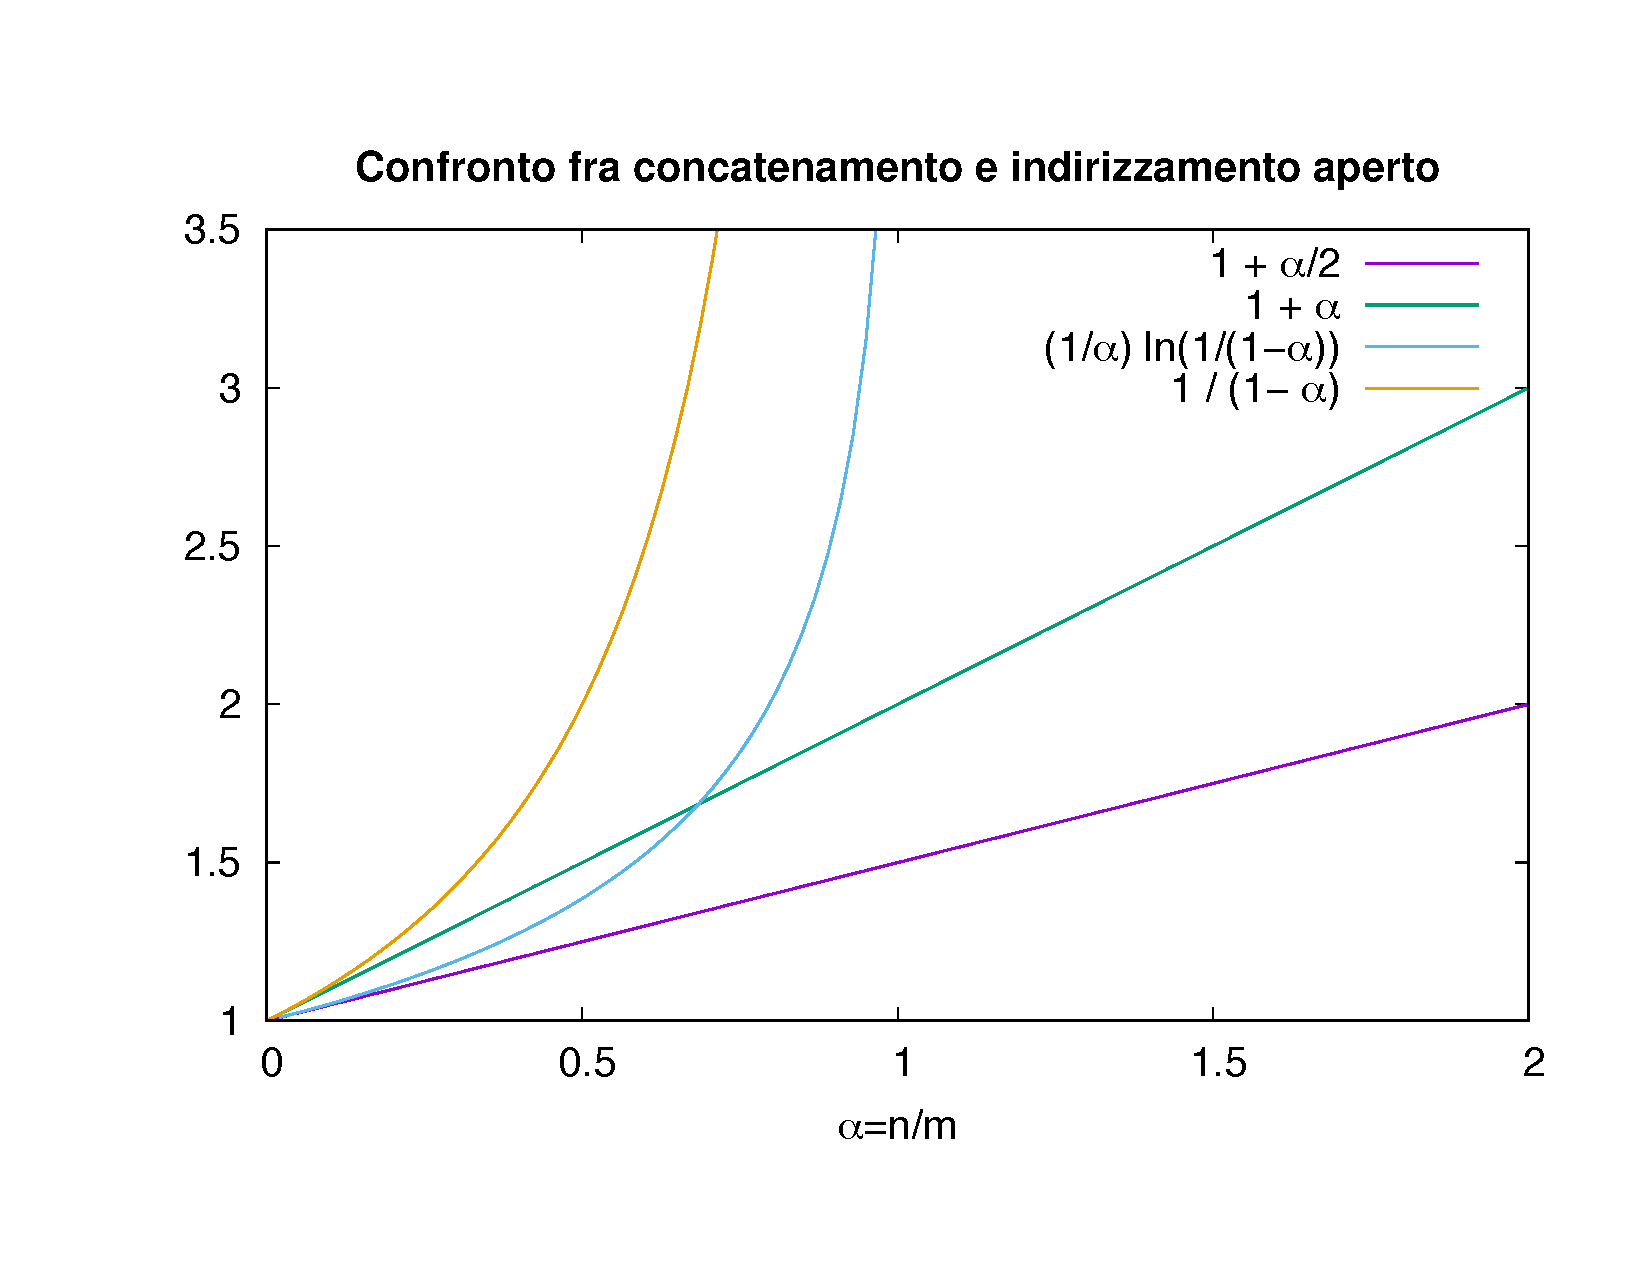
\includegraphics{graphs/ConfrontoTecnicheHash.pdf}
\end{figure}

{Notiamo che i costi del concatenamento con indirizzamento aperto (giallo e azzurro) crescono molto più velocemente rispetto alle liste di collisione (viola e verde).}


%mod 2

\chapter{Grafi}

{Coppia ordinata $G=(V,E)$ formata da due insiemi $V$ (vertici) ed $E$ (archi)}

$V = \{1,2,3,\ldots,n\}$

{$E \subseteq VxV$, ovvero $E$ è un sottoinsieme dell'insieme delle parti (prodotto cartesiano) dell'insieme $V$}

{I grafi possono essere}

\begin{itemize}
\tightlist
\item
  {Orientati}
\item
  {Non orientati, se le relazioni sono simmetriche}
\end{itemize}

{~~~~~~~~se $\forall(u,v) \in E \iff (v,u) \in E$}

{Non si ammettono cappi nei grafi non orientati.}

$\forall u \in E \iff (u,u) \notin E$

\section{Sottografi}

{Sottografo di $G$}

{$G'=(V',E')$ è sottografo di $G$ se $V'\subseteq V$ e $E'\subseteq E$}

\paragraph{Sottografo indotto}

{Dato $V' \subseteq V$, il sottografo indotto da $V'$ di $G$ è $G[V']=(V',E')$, con $E' = E\,\cap\,V\,x\,V'$}

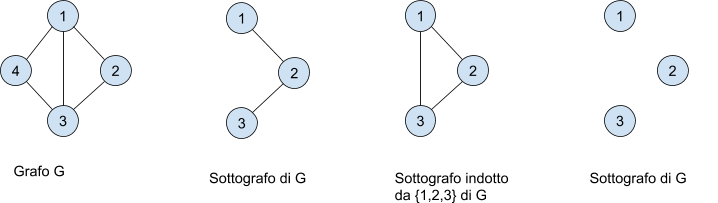
\includegraphics{images/image534.png}

\section{Cammini}

{Un cammino di $G$ è una sequenza $<X_0,X_1,\ldots,X_k>$ dove i vertici appartengono al grafo di partenza.}

$\forall i,0\leq i\leq k,(X_i,X_{i+1})\in E$

\subsection{Cammini semplici e cammini non semplici}

$<1,2,3,4,5>$ è un cammino semplice\\
$<1,2,3,1,4,5>$ non è un cammino semplice

{Un cammino è semplice se tutti i vertici sono distinti}

\paragraph{Lunghezza di un cammino}

{La lunghezza di un cammino è il numero dei suoi archi}

\paragraph{Raggiungibilità dei vertici}

$u$ è raggiungibile da $v$ se esiste un cammino $<X_0,X_1,X_2,\ldots,X_k>$ tale che $X_0 = u$ e $X_k = v$

\paragraph{Ciclo}

{Un ciclo è un cammino dove $X_0 = X_k$}

{Un grafo senza cicli si dice aciclico.}

\paragraph{{[}NO{]}Grafo connesso}

{Un grado non orientato si dice connesso se $\forall (u,v) | u,v \in V$, esiste un cammino da $u$ a $v$ con $u\neq v$}

\paragraph{{[}NO{]} Componente connessa}

{Dato $G=(V,E)$ e $V' \subseteq V$}

{$V'$ si dirà componente connessa se }

\begin{enumerate}
\tightlist
\item
  {$G[V']$ è connesso}
\item
  $V'${~non è sottoinsieme stretto di un sottografo connesso}
\end{enumerate}

{Se il numero di componenti connesse di un grafo è uguale a 1, }{il
grafo è connesso.}

\paragraph{{[}NO{]}Vertici adiacenti}

{Dato $G=(V,E)$ e $u \in V$}

{Il grado di $u$, $deg(u)$ è il numero di vertici adiacenti a $u$}

\paragraph{Arco incidente}

{Un arco che è collegato ad $v$}

\paragraph{Vertici isolati e terminali}

{Se $deg(u) = 0$ allora $u$ è isolato}

{Se $deg(u) = 1$ allora $u$ è terminale}

\section{Teorema della stretta di mano (HandShaking Lemma)}


\begin{lemma}{Teorema della stretta di mano}{handshaking_Lemma}

{{[}NO{]}}

\begin{equation}
\sum_{u \in V}{degree(u)} = 2m
\end{equation}

{dove $m = \abs{E}$ è il numero di archi.}

{{[}O{]}}

{$outDegree(u)$ : numero degli archi uscenti da $u$}

{$inDegree(u)$ : numero degli archi entranti in $u$}

\begin{equation}
\sum_{u \in V}{outDegree(u)} = \sum_{u \in V}{inDegree(u)} = m
\end{equation}

\end{lemma}



{{[}NO{]} Proprietà}

{Il numero di vertici che hanno grado dispari è sempre pari}

\paragraph{Dimostrazione}

$V=P\cup D$

$P = \{u \in V | deg(u) \, pari\}$

$D = \{u \in V | deg(u) \, dispari\}$

$2m = \sum_{u \in V}{deg(u)} = \sum_{u \in P}{deg(u)} + \sum_{u \in D}{deg(u)}$

$2m = \sum_{u \in P}{2*h(u)} + \sum_{u \in D}{2*h(u)+1}$

$2m = \sum_{u \in P}{2*h(u)} + \sum_{u \in D}{2*h(u)} + \abs{D}$

$\abs{D} = 2m - 2 *\sum_{u \in P}{h(u)} + 2*\sum_{u \in D}{h(u)}$

$\abs{D} = 2*(m-\sum_{u \in V}{h(u)})$

{Il numero di vertici con grado dispari è quindi pari}

\paragraph{Esercizio}
{~~~~~~~~Dimostrare che, dato $G=(V,E)$ non orientato senza vertici isolati (nessuno vertice ha grado 0),}

{~~~~~~~~con $\abs{E} = \abs{V} -1$}

{Allora, esistono almeno due vertici terminali}

{Dimostrazione per assurdo:}

$n=\abs{V},m=\abs{E}$

{Per il lemma della stretta di mano:}

$\sum_{u \in V}{deg(u)} = 2$ e $\abs{E} = 2m$

$2n-2 = 2m = \sum_{u \in V}{deg(u)}$

{Chiamo $V_1$ un sottoinsieme di $V$ di vertici terminali}

$V_1=\{u\in V\,|\,deg(u)=1\}$

{Il problema diventa: dimostrare che $\abs{V_1} \geq 2$}

$2m = \sum_{u \in V_1}{deg(u)} +  \sum_{u \in V \setminus V_1}{deg(u)}$

$2n -2 \geq 2n - \abs{V_1}$

{????}\textsuperscript{\protect\hyperlink{cmnt21}{{[}u{]}}}

{$\abs{V_1} \geq 2$ OK}

\section{Matrice di adiacenza}

{Dato $G=(V,E)$}

$n=\abs{V},m=\abs{E}$

{$A$ Matrice quadrata $n x n$ }

\begin{itemize}
\tightlist
\item
  {Per trovare il grado di un vertice basta calcolare la somma degli elementi sulla corrispondente riga}
\item
  {{[}NO{]} $n$ archi in totale = doppia somma di tutti gli elementi della matrice}
\item
  {{[}O{]} $n$ archi in totale = doppia somma di tutti gli elementi della matrice}
\end{itemize}

{Usare le matrici di adiacenza solitamente conviene se ci sono molti archi, altrimenti è meglio utilizzare le liste.}

\paragraph{Matrice di adiacenza per grafi orientati}

\begin{equation}
A_{i,j} = 
\begin{cases}
0 & \mbox{se } (i,j) \notin E \\ 
1 & \mbox{se } (i,j) \in E
\end{cases}
\end{equation}

{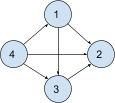
\includegraphics{images/image529.png}}

\begin{tabular}{|c|c|c|c|c|}
\hline 
  & \textbf{1} & \textbf{2} & \textbf{3} & \textbf{4} \\ 
\hline 
\textbf{1} & 0 & 1 & 1 & 0 \\ 
\hline 
\textbf{2} & 0 & 0 & 0 & 0 \\ 
\hline 
\textbf{3} & 0 & 1 & 0 & 0 \\ 
\hline 
\textbf{4} & 1 & 1 & 1 & 0 \\ 
\hline 
\end{tabular} 

\paragraph{Matrice di adiacenza per grafi non orientati}

\begin{equation}
A_{i,j} = 
\begin{cases}
0 & \mbox{se } \{i,j\} \notin E \\ 
1 & \mbox{se } \{i,j\} \in E
\end{cases}
\end{equation}

{Essendo la relazione tra vertici simmetrica, $A=A^T$ (trasposta)}

{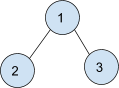
\includegraphics{images/image535.png}}

\begin{tabular}{|c|c|c|c|}
\hline 
  & \textbf{1} & \textbf{2} & \textbf{3} \\ 
\hline 
\textbf{1} & 0 & 1 & 1 \\ 
\hline 
\textbf{2} & 1 & 0 & 0 \\ 
\hline 
\textbf{3} & 1 & 0 & 0 \\ 
\hline 
\end{tabular} 

\section{Liste concatenate}

{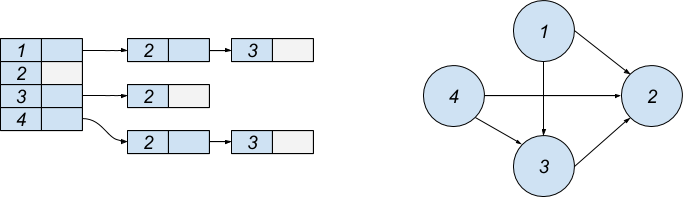
\includegraphics{images/image537.png}}

{Usare le liste di adiacenza solitamente conviene se ci sono pochi archi, altrimenti è meglio utilizzare le matrici.}

{{[}O{]} Densità}

\begin{equation}
\delta=\frac{numero\,di\,archi}{numero\,di\,possibili\,archi} = \frac{numero\,di\,archi}{n^2}
\end{equation}

$n=\abs{V},m=\abs{E}$

$\delta=\frac{m}{n^2}$

\paragraph{{[}NO{]} Densità}

\begin{equation}
\delta=\frac{numero\,di\,archi}{numero\,di\,possibili\,archi}
\end{equation}

{$\delta=\frac{m}{k},\,k = \frac{n(n-1)}{2}$ coefficiente binomiale}


{Grafi sparsi ($n\simeq m$): lista}

{Grafi densi ($n^2\simeq m$): matrice}

\paragraph{Proprietà}

{Sia $G$ un grafo NO. Se $G$ è aciclico, allora la cardinalità $\abs{E} \leq \abs{V}-1$}

\paragraph{ Dimostrazione induttiva su $n=\abs{V}$}

{~~~~~~~~Caso base:}

{~~~~~~~~~~~~~~~~se $n=1$ allora $m = 0$

{~~~~~~~~~~~~~~~~se $n=2$ allora $m \leq 1$

{~~~~~~~~Passo induttivo $n \geq 3$:}


\paragraph{{[}NO{]} Complemento di un grafo}

{Il complemento di un grafo è un grafo con gli stessi vertici, i cui archi sono complementari:}

$G=(V,E), \overline{G}=(\overline{V},\overline{E})$

\section{Grafo autocomplementare}

{Un grafo è detto autocomplementare se $\overline{G}=G$ ovvero se $\forall(i,j) \in E\,sse\,(i,j) \in \overline{E}$}

{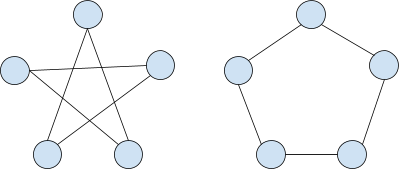
\includegraphics{images/image532.png}}

\subsection{Prodotto tra matrici di adiacenza}

\subsubsection{Prodotto di matrici}

{Due matrici $n\,x\,m$ ed $p\,x\,n$ (il numero di righe della prima equivale al numero di colonne della seconda) possono essere moltiplicate tramite il prodotto ``righe per colonne''.}

$C = A*B$ \\
$C_{i,j}=\sum_{k=1}^{n}{a_{i,k}*a_{k,j}}$

\subsubsection{Matrice al quadrato}


{Moltiplicando una matrice di adiacenza $A$ per se stessa, tramite il prodotto tra righe e colonne, ottengo una matrice delle stesse dimensioni con le seguenti caratteristiche:}

\begin{itemize}
\tightlist
\item
  {Sulla diagonale principale ho i gradi dei vertici}
\item
  {Nelle altre posizioni ho il numero di cammini tra i e j di lunghezza
  2}
\end{itemize}

$A^2 = A*A = (a^{(2)}_{i,j})$ \\
$a^{(2)}_{i,j}=\sum_{k=1}^{n}{a_{i,k}*a_{k,j}}$

\paragraph{Dimostrazione}

{``Sulla diagonale principale ho i gradi dei vertici'' ($i=j$)}

$a^{(2)}_{i,j}=\sum_{k=1}^{n}{a_{i,k}*a_{k,i}}$

{Essendo $G$ non orientato, la matrice è simmetrica e $a_{i,k}*a_{k,i} = a^2_{i,k}$}

{$a^{(2)}_{i,i} = \sum^n_{k=1}{a^2_{i,k}}$ , notiamo che il termine della sommatoria contiene solo valori binari che elevati al quadrato restituiscono il medesimo valore. Perciò}

$a^{(2)}_{i,i} = \sum^n_{k=1}{a^2_{i,k}} = \sum^n_{k=1}{a_{i,k}} = deg(i)$

{``Nelle altre posizioni ho il numero di cammini tra $i$ e $j$ di lunghezza'' ($i\neq j$)}

{$a^2_{i,j}=\sum_{k=1}^{n}{a_{i,k}*a_{k,j}}$, essendo la matrice di adiacenza composta da valori binari, il prodotto risulta valere 1 solo se entrambi i fattori valgono 1, ovvero se esiste un cammino di lunghezza 2}

\subsubsection{Matrice con esponente maggiore di 2}

{$A^n, n > 2$ conterrà}

\begin{itemize}
\tightlist
\item
  {Sulla diagonale: il numero di cicli di lunghezza n che partono da i}
\item
  {Fuori dalla diagonale: il numero di cammini di lunghezza n}
\end{itemize}

{Dimostrazione per induzione:}\textsuperscript{\protect\hyperlink{cmnt22}{{[}v{]}}\protect\hyperlink{cmnt23}{{[}w{]}}}

{Ipotesi:}

{~~~~~~~~Passo induttivo:}

$A^n = A *A* A * \ldots * A$ ($n$ volte) $=A^{n-1}*A$

{$a_{i,j^{(n)}} = \sum_{k=1}^n{a^{(n-1)}_{i,k}*a_{k,j}}$, ovvero il numero di cammini da $i$ a $j$ passanti per $k$.}

{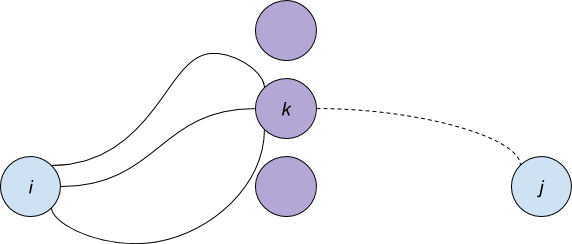
\includegraphics{images/image538.png}}

\paragraph{Esercizio}

{Mostrare che $G=(V,E) [NO]$ contiene un triangolo, ovvero un ciclo di lunghezza 3, se e solo se esistono due indici $i,j$ tali che sia la matrice di adiacenza $A$ e la matrice al quadrato $A^2$ hanno un elemento non nullo in posizione $(i,j)$}

\section{{[}NO{]} Grafi regolari}

{$G=(V,E)$ si dice k-regolare se tutti i vertici hanno grado $k$. Con $n=\abs{V},m=\abs{E}$}

{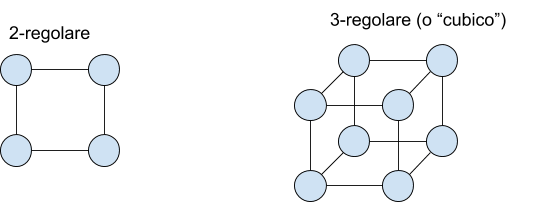
\includegraphics{images/image524.png}}

\paragraph{Proprietà}

{Se $G$ è 2-regolare allora il numero di vertici coincide necessariamente con il numero degli archi. $n=m$}

\paragraph{Dimostrazione}

{Utilizziamo il teorema della stretta di mano}

$2m=\sum_{u\in V}{deg(u)}$\textsuperscript{\protect\hyperlink{cmnt24}{{[}x{]}}\protect\hyperlink{cmnt25}{{[}y{]}}}

\paragraph{Esercizio}

{Dimostrare che se il grafo $G$ è 3-regolare, allora $n$ è pari. Analogamente, analizzare $G$ 4-regolare. }

\section{Isomorfismi di grafi}

{Un isomorfismo di grafi è un funzione che mappa un grafo in un secondo dalla stessa forma.}

{Viene fornita la definizione per i grafi non orientati, essa può però essere adattata a grafi orientati.}

\paragraph{{[}NO{]} Definizione}

$G_1=(v_1,E_1),G_2(V_2,E_2)$

{$\Theta:V_1\rightarrow V_2$ si dice isomorfismo se valgono le due proprietà:}

\begin{enumerate}
\tightlist
\item
  {$\Theta$ deve essere una funzione biettiva (è necessaria una corrispondenza 1-1).}
\item
  {La relazione di adiacenza deve essere preservata\\
  $\forall u,v \in V_1, (u,v) \in E_1 \iff (\Phi(u),\Phi(v)) \in E_2$}
\end{enumerate}

\subsection{Determinare se due grafi sono isomorfi}

{$G_1=(v_1,E_1),G_2(V_2,E_2)$ sono isomorfi se esiste un isomorfismo da $G_1$ a $G_2$ e si indica con $G_1\simeq G_2$}

{Condizioni necessarie perché $G_1\simeq G_2$:}

\begin{enumerate}
\tightlist
\item
  $\abs{V_1}=\abs{V_2}$
\item
  $\abs{E_1}=\abs{E_2}$
\item
  {Stessa degree sequence $degseq(G_1) = degseq(G_2)$}
\item
  $\#ComponentiConnesse(G_1) = 	\#ComponentiConnesse(G_2)$
\end{enumerate}


\begin{longtable}[]{@{}lll@{}}
\toprule
\begin{minipage}[t]{0.30\columnwidth}\raggedright\strut
$G$\strut
\end{minipage} & \begin{minipage}[t]{0.30\columnwidth}\raggedright\strut
$\overline{G}$\strut
\end{minipage} & \begin{minipage}[t]{0.30\columnwidth}\raggedright\strut
{Può verificarsi?}\strut
\end{minipage}\tabularnewline
\begin{minipage}[t]{0.30\columnwidth}\raggedright\strut
{Connesso}\strut
\end{minipage} & \begin{minipage}[t]{0.30\columnwidth}\raggedright\strut
{Connesso}\strut
\end{minipage} & \begin{minipage}[t]{0.30\columnwidth}\raggedright\strut
{FALSO}\strut
\end{minipage}\tabularnewline
\begin{minipage}[t]{0.30\columnwidth}\raggedright\strut
{Connesso}\strut
\end{minipage} & \begin{minipage}[t]{0.30\columnwidth}\raggedright\strut
{Disconnesso}\strut
\end{minipage} & \begin{minipage}[t]{0.30\columnwidth}\raggedright\strut
{FALSO \\ (Es: autocomplementare)}\strut
\end{minipage}\tabularnewline
\begin{minipage}[t]{0.30\columnwidth}\raggedright\strut
{Disconnesso}\strut
\end{minipage} & \begin{minipage}[t]{0.30\columnwidth}\raggedright\strut
{Connesso}\strut
\end{minipage} & \begin{minipage}[t]{0.30\columnwidth}\raggedright\strut
{VERO}\strut
\end{minipage}\tabularnewline
\begin{minipage}[t]{0.30\columnwidth}\raggedright\strut
{Disconnesso}\strut
\end{minipage} & \begin{minipage}[t]{0.30\columnwidth}\raggedright\strut
{Disconnesso}\strut
\end{minipage} & \begin{minipage}[t]{0.30\columnwidth}\raggedright\strut
{FALSO}\strut
\end{minipage}\tabularnewline
\bottomrule
\end{longtable}

{Il problema di determinare l'esistenza di un'isomorfismo tra due grafi è esoso in termini di tempo. Per evitare il bruteforce di tutte le combinazioni si procede a mappare gli archi con grado analogo.}

\section{Grafi planari}

Un grafo è planare se tutti archi non sono incidenti.

\begin{teorema}{Clique su grafi planari}{theoexample}
Le clique sui grafi planari hanno $k <= 4$. Con valori maggiori di 4 non è più possibile costruire clique su grafi planari.
\end{teorema}


\chapter{Albero di copertura minimo (MST)}

{Sia $T$ un albero di copertura,definisco}

$w(T) = \sum_{(u,v)\in T}{w(u,v)}$

{dove $w:E\rightarrow \mathbb{R}$ è detta ``funzione peso''}

{Definizione:}

{Un albero di copertura }$T${~si dice minimo o ``di peso minimo'' (minimum spanning tree) se $w(T)$ è il minimo rispetto a tutti gli alberi di copertura}


\section{Teorema fondamentale degli MST}

\begin{teorema}{Teorema fondamentale degli MST}{mst_theorem}
{Sia $G=(V,E) [NO]$ connesso con funzione peso $w$.}

{Se le tre condizioni}

\begin{enumerate}
\tightlist
\item
  {$A \subseteq E$ è contenuto in qualche MST}
\item
  {$(S,V \setminus S)$ è un taglio che rispetta $A$}
\item
  {Sia $(u,v)$ un arco leggero che attraversa il taglio $(S,V \setminus S)$}
\end{enumerate}

{sono rispettate, allora l'arco $(u,v)$ è sicuro per $A$, ovvero $A \subseteq \{(u,v)\}$ è contenuto in qualche MST.}

\end{teorema}

\paragraph{Dimostrazione}

{$A \subseteq T$ con $T$ MST}

{Due casi:}

\begin{enumerate}
\tightlist
\item
  {$(u,v) \in T$, caso banale in quanto $A \cup \{(u,v)\} \subseteq T$  e $T$ è l'MST che cerchiamo.}
\item
  {$(u,v) \notin T$, quindi $T$ non è l'MST che cerchiamo, procediamo quindi a costruirne uno:}
\end{enumerate}

{Per le sei proprietà fornite, se unisco $(u,v)$ a $T$ formo un ciclo, è quindi necessario rimuovere l'altro cammino $(x,y)$ che lo forma tra gli archi che attraversano il taglio. }

$T' = T \cup {(u,v)} \setminus \{(x,y)\} $

\begin{figure}[H]
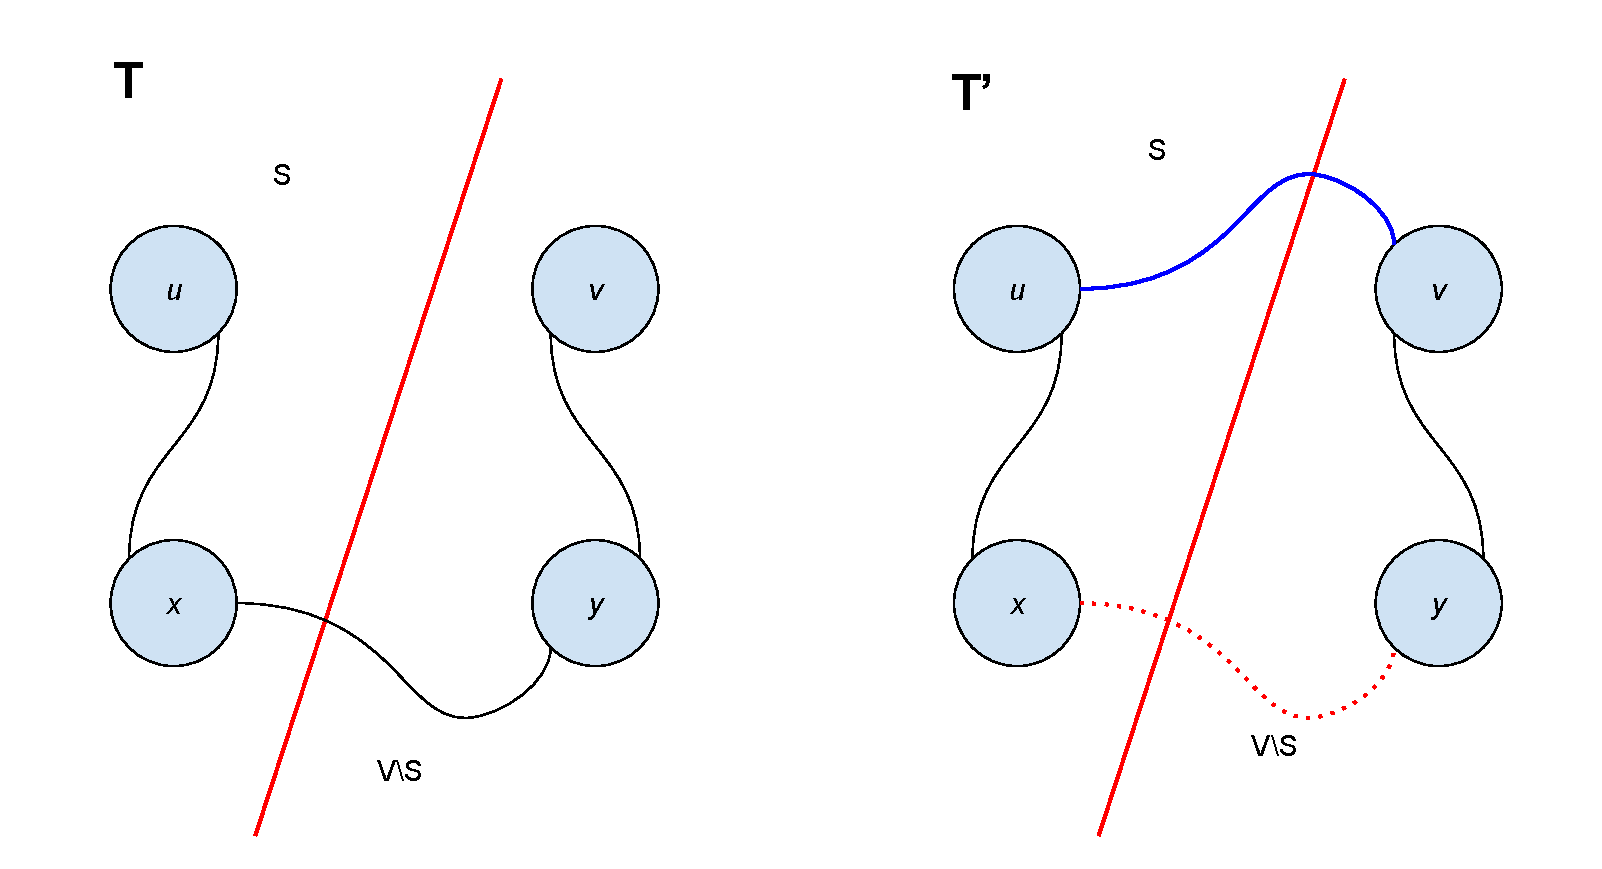
\includegraphics{graphs/arco_taglio_leggero.pdf}
\end{figure}

$w(u,v) \leq w(x,y)${: Il peso dell'arco aggiunto è minore del peso dell'arco rimosso, in quanto esso è leggero per ipotesi.}

{Quanto vale allora $w(T')$? }

$w(T') \leq w(T)$ {ed essendo }$w(u,v) \leq w(x,y)${~allora $w(T') \leq w(T)$}

{Da }$w(T) \leq w(T') \leq w(T)$ \textsuperscript{\protect\hyperlink{cmnt26}{{[}z{]}}}{risulta che $w(T') = w(T)$, e }$T'${~è quindi un MST.}

{Nota}\textsuperscript{\protect\hyperlink{cmnt27}{{[}aa{]}}}{: se $w(u,v) = w(x,y)$ allora $(u,v) = (x,y)$?}

{Dobbiamo però dimostrare che $T'$ sia ``sicuro'', e perciò dimostriamo che \\ $A \cup \{(u,v)\} \subseteq T'$}

\paragraph{Corollario}

{Sia $G=(V,E) [NO]$ connesso con funzione peso $w$. Se le tre condizioni}

\begin{enumerate}
\tightlist
\item
  {$A \subseteq E$ è contenuto in qualche MST}
\item
  {$C$ è una componente connessa della foresta $(V,A)$}
\item
  {Sia $(u,v)$ un arco leggero che collega la componente $C$ con il resto del grafo}
\end{enumerate}

{sono rispettate, allora l'arco $(u,v)$ è sicuro per $A$, ovvero $A \cup \{(u,v)\}$ è contenuto in qualche MST.}

\paragraph{Dimostrazione}

{Se impongo che}

\begin{itemize}
\tightlist
\item
  {Il taglio dell'ipotesi 2 sia $(C,V\setminus C)$, in modo da isolare la componente connessa}
\item
  {MANCA}\textsuperscript{\protect\hyperlink{cmnt28}{{[}ab{]}}}
\end{itemize}

{posso utilizzare il teorema fondamentale per la dimostrazione}

\paragraph{Corollario}

{Sia $(u,v)$ un arco di peso minimo in $G$. Allora $(u,v)$ appartiene a qualche MST.}

\subsubsection{Dimostrazione tramite la tecnica ``cuci e taglia''}

{Sia T un MST di G. }

{Due casi:}

\begin{enumerate}
\tightlist
\item
  $(u,v)\in T${, ovvio}
\item
  $(u,v)\notin T$
\end{enumerate}

\paragraph{Corollario}

{Sia $(u,v)$ un arco di peso minimo in $G$ e supponiamo che sia unico. Allora $(u,v)$ appartiene a tutti gli MST}\textsuperscript{\protect\hyperlink{cmnt29}{{[}ac{]}}}{.}

\paragraph{Dimostrazione per assurdo}

{Nonostante le ipotesi, esiste {[}almeno{]} un MST senza l'arco in
questione.}

{Non esistendo, provvediamo ad aggiungerlo a T. $T' = T \cup \{(u,v)\}$}

{Facendo ciò creo sicuramente un ciclo, in quanto $T$ è albero. Scelto un arco $(x,y)$ e lo rimuovo. Ho quindi costruito un albero di copertura con peso $W(T') = W(T) + w(u,v) - w(x,y) < W(T)$}

{Con $w(u,v) < w(x,y)$ (minore stretto!)}

{Contraddizione}{: essendo T MST, non può esistere un altro albero con peso inferiore.}

\paragraph{Esercizio}

$G=(V,E) [NO]$ connesso con $w:E \rightarrow \mathbb{R}$

{Sia $T_{min}$ un MST di G.}

{Sia $T'$ un albero di copertura (ST) non necessariamente minimo (M).}

{Siano $(u,v),(x,y)$ rispettivamente gli archi di $T,T'$ di peso massimo. Ordino gli archi e considero i pesi maggiori.}

$T_{min}: <e_1,e_2,\ldots,e_{n-1}>$ con $e_{n-1} = (u,v)$

$T': <e'_1,e'_2,\ldots,e'_{n-1}>$ con $e'_{n-1} = (x,y)$

{Congettura: $w(u,v) \leq w(x,y)$}

{Si può procedere per confutazione con controesempio oppure per dimostrazione tramite metodo ``cuci e taglia''.}

{Soluzione}\textsuperscript{\protect\hyperlink{cmnt30}{{[}ad{]}}}{:}

\paragraph{Esercizio}

{Dimostrare che, se tutti i pesi del grafo sono distinti, allora esiste un solo MST.}

{Soluzione}\textsuperscript{\protect\hyperlink{cmnt31}{{[}ae{]}}}{:}

\section{Generazione degli alberi di copertura minima}

\lstinputlisting{code/generic_mst.txt}

{Verranno analizzati gli algoritmi di Kruskal e Prim, i quali differiscono per l'implementazione della ricerca dell'arco sicuro.}

{Kruskall utilizza le strutture dati Set per la gestione di insiemi disgiunti. Esse dispongono di tre operatori:}

\begin{enumerate}
\tightlist
\item
  {Make\_set(X)}
\item
  {Union(x,y) o Merge\_set(x,y)}
\item
  {Find\_set(x)}
\end{enumerate}

{Esempio di utilizzo: determinare le componenti connesse di un grafo}

\lstinputlisting{code/componenti_connesse.txt}


\subsubsection{Simulazione di esecuzione}

\paragraph{Tramite grafo}

%{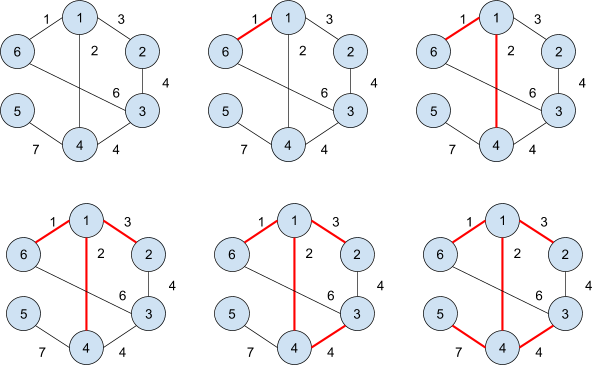
\includegraphics{images/image519.png}}
\begin{figure}[H]
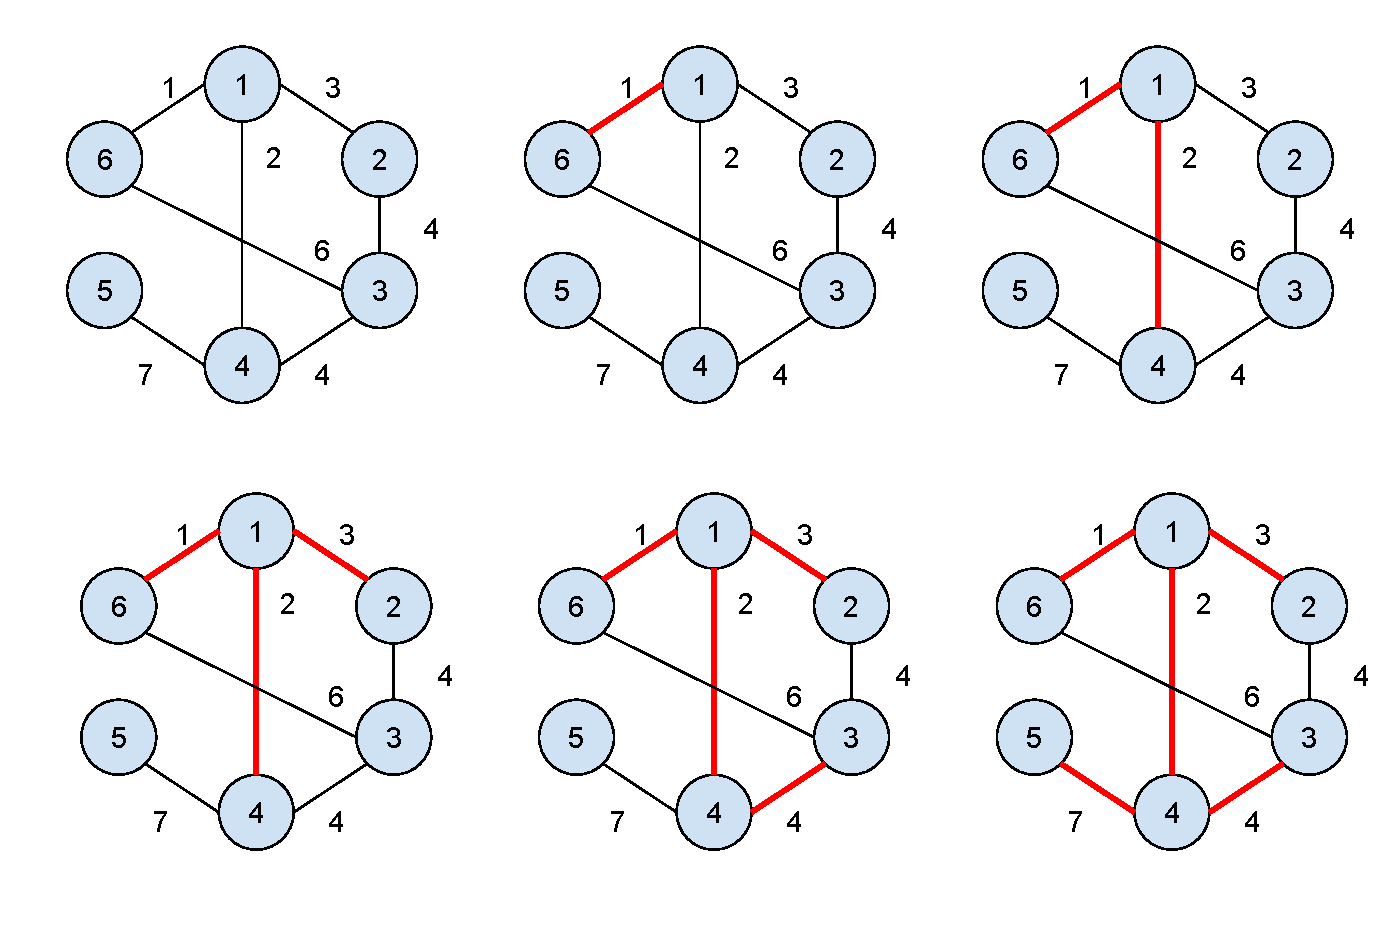
\includegraphics{graphs/simulazione_grafo.pdf}
\end{figure}


\paragraph{Tramite tabella}

\begin{tabular}{|l|l|l|}
\hline 
Passo & A & Insiemi disgiunti \\ 
\hline 
1 & $\{\}$ & $\{1\},\{2\},\{3\},\{4\},\{5\},\{6\}$ \\ 
\hline 
2 & $\{(1,6)\}$ & $\{1,6\},\{2\},\{3\},\{4\},\{5\}$ \\ 
\hline 
3 & $\{(1,6),(1,4)\}$ & $\{1,4,6\},\{2\},\{3\},\{5\}$ \\ 
\hline 
4 & $\{(1,6),(1,4),(1,2)\}$ & $\{1,2,4,6\},\{3\},\{5\}$ \\ 
\hline 
5 & $\{(1,6),(1,4),(1,2),(4,3)\}$ & $\{1,2,3,4,6\},\{5\}$ \\ 
\hline 
6 & $\{(1,6),(1,4),(1,2),(4,3),(4,5)\}$ & $\{1,2,3,4,5,6\}$ \\ 
\hline 
\end{tabular} 

\subsection{Generazione di MST : Kruskal}

$G=(V,E)$ connesso, $n=\abs{V},m=\abs{E}$

\lstinputlisting{code/kruskal.txt}

{*Per l'analisi delle due find\_set e della union ci viene fornita la complessità ottenuta tramite Heichmann.\\
}{Complessità}{:}

{$O(mlog(m)+n+mlog(m))$, avendo $m \geq n-1$ archi poichè l'arco è connesso, la complessità è $O(mlog(m))$}


\subsection{Generazione di MST : Prim}

{A differenza di Kruskal, Prim richiede un vertice di partenza detto ``radice''. Con l'insieme Q si indica l'insieme dei vertici da estrarre.
$V\setminus Q$ indica quindi l'insieme dei vertici già estratti. $Q$ è una coda di priorità, implementata tramite Heap Binario, i cui elementi hanno le seguenti caratteristiche:}

\begin{itemize}
\tightlist
\item
  Predecessore: $\pi[u]$
\item
Chiave: $Key[u]$ valore dell'arco incidente che attraversa il taglio $(Q,Vsetminus Q)$ con peso minore. Si utilizza il valore infinito positivo per indicare l'eventuale assenza di archi.
\end{itemize}

\lstinputlisting{code/prim.txt}

La convergenza risulta essere finita

La complessità della funzione Prim è $O(m logn)$

{Simulazione}

{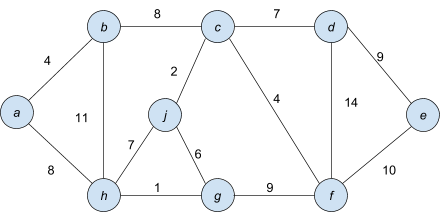
\includegraphics{images/image542.png}}


\chapter{Cammini minimi}

{Solitamente si sottintende l'utilizzo su grafi orientati, in caso di grafi non orientati, ogni arco può essere sostituito da una coppia di archi inversamente orientati.}

$G=(V,E,w)$ orientato, $w:E\rightarrow \mathbb{R}$

Un cammino $p$ è una sequenza $<x_0,x_1,\ldots,x_q>$, $\forall i, i\leq i \leq q, (x_{i-1},x_i) \in E$.

$w(p)=\sum_{i=1}^{q} w(x_{i-1},x_i)$ è la funzione ``peso'' di un cammino $p$.

{La distanza $\delta(u,v)$ tra due vertici $u,v \in V$ è definita nel seguente modo:}

{$\delta(u,v) = +\infty$ se non esiste un cammino orientato da u a v}

{$\delta(u,v)=min(w(p))$ minimo dei pesi dove $p$ è il cammino tra $u$ e $v$}

\paragraph{Varianti}

{Esistono quattro diverse varianti di ricerca dei cammini minimi, combinazioni dei due casi di numerosità dei vertici di partenza e di destinazione.}

\begin{table}[]
\centering
\begin{tabular}{ll|l|l|}
\cline{3-4}
                                                 &                               & \multicolumn{2}{c|}{Destinazione}                            \\ \cline{3-4}
                                                 &                               & \multicolumn{1}{c|}{Singola} & \multicolumn{1}{c|}{Multipla} \\ \hline
\multicolumn{1}{|c|}{}                           & \multicolumn{1}{c|}{Singola}
& \specialcell{In: $G(V;E;w)\,u,v\in V$\\Out: $\delta(u,v)$ }
& \cellcolor[HTML]{F8A102}\specialcell{In: $G(V;E;w)\,s\in V$\\Out: $\forall v \in V, \delta(s,v)$}   \\ \cline{2-4}
\multicolumn{1}{|c|}{\multirow{-2}{*}{Sorgente}} & \multicolumn{1}{c|}{Multipla}
& \specialcell{In: $G(V;E;w)\,d\in V$\\Out: $\forall v \in V, \delta(v,d)$}
& \cellcolor[HTML]{F8A102}\specialcell{In: $G(V;E;w)$\\Out: $\forall u,v \in V, \delta(u,v)$}    \\ \hline
\end{tabular}
\end{table}

{Solo i casi evidenziati verranno presi in analisi, in quanto gli altri due sono sottoproblemi di essi.}

\paragraph{Archi con pesi negativi}

{Ci domandiamo se sia possibile risolvere il problema degli archi con peso negativo sommando ai pesi di tutti gli archi del grafo $G$ la costante $k$ capace di renderli tutti positivi. Es: $k=-min(w(u,v))\,\forall u,v \in E$}

{NO. Sommare una costante ai pesi degli archi altera eventuali somme di pesi di archi di lunghezza differente in maniera diversa.}

\section{Cammini minimi con sorgente singola}

\subsection{Strutture dati per la rappresentazione dei cammini minimi}

{Per ogni vertice $u \in V$ necessitiamo di due campi:}

\begin{enumerate}
\tightlist
\item
$d[u]$ : stima della distanza tra $s$ ed $u$
\item
$\pi[u]$ : predecessore
\end{enumerate}

\subsection{Sottografo dei predecessori}

{Dato $G=(V,E,w)$, il sottografo dei predecessori è $G_\pi=(V_\pi,E_\pi)$ dove}

$V_\pi=\{u \in V | \pi[u] \neq NIL\} \cup \{s\}$ : Lista dei vertici già estratti

$E_\pi=\{(\pi[u],u) \in E | u \in V_{\pi} \setminus \{s\}\}$ : Lista degli archi tra i vertici già estratti

\subsection{Albero dei cammini minimi}

{Dato $G=(V,E,w)$, l'albero dei cammini minimi $G'=(V',E')$ è un sottografo di $G$ dove}

{$V'$ : tutti gli archi raggiungibili dal vertice sorgente}

{$G'$ : forma un albero radicato in $s$}

{$\forall v \in V'$ l'unico cammino tra $s$ e $v$ in $G'$ è un cammino minimo in $G$}

\subsection{Procedure di modifica dei due campi}

\paragraph{Init single source}

\lstinputlisting{code/init_single_source.txt}

\paragraph{Relax}

La relax è una procedura che aggiorna i valori  delle distanze dei vertici dall'origine.

\begin{tikzpicture}[>=stealth, every node/.style={circle, draw, minimum size=0.75cm}]
\graph [tree layout, grow=down, fresh nodes, level distance=0.5in, sibling distance=0.5in]
    {
        4 -> { 
          3 -> { 1 -> { 5, " " }, 2,2 },
          3 -> { 1, 2, 2 },
          3 -> { 1, 2, 2 }
        } 
    };
\end{tikzpicture}

\lstinputlisting{code/relax.txt}

\subsection{Dijkstra}

\lstinputlisting{code/dijkstra.txt}

{La coda di priorità $Q$ può essere implementata tramite}

\begin{enumerate}
\tightlist
\item
  {Array lineare}
\item
  {Heap binario}
\end{enumerate}

\paragraph{Complessità}

Notiamo che la Relax viene eseguita $\sum_{u \in V}{outDeg(u)} = m$ volte e non $n^2$.

\paragraph{Array Lineare}

{Studiamo la complessità di Dijkstra con coda di priorità implementata tramite array lineare:}

La fase di inizializzazione è complessa $O(n)$. \\
ExtractMin è complessa $O(n)$, essendo dentro al ciclo di $n$ ripetizioni, la complessità totale sarà $O(n^2)$. \\
Relax è complessa $O(1)$ e, nonostante sia dentro al ciclo, viene eseguita $m$ volte per una complessità totale di $O(m)$.

La complessità totale è $O(n+n^2+m)$, il cui termine prevalente $n^2$ determina la complessità $O(n^2)$.

\paragraph{Heap Binario}

{Studiamo la complessità di Dijkstra con coda di priorità implementata tramite heap binario:}

La fase di inizializzazione è complessa $O(n)$. \\
ExtractMin è complessa $O(log(n))$, essendo dentro al ciclo di $n$ ripetizioni, la complessità totale sarà $O(n*log(n))$. \\
Relax è complessa $O(log(n))$ e, nonostante sia dentro al ciclo, viene eseguita $m$ volte per una complessità totale di $O(m*log(n))$.

La complessità totale è $O(n+n*log(n)+m*log(n))$, il cui termine prevalente $m*log(n)$ determina la complessità $O(m*log(n))$.

\paragraph{Conclusioni}

\begin{table}[h]
\centering
\caption{Complessità}
\begin{tabular}{ll|l|l|}
\cline{3-4}
                                                        &                                      & \multicolumn{2}{c|}{\textbf{Implementazione}}                                            \\ \cline{3-4}
                                                        &                                      & \multicolumn{1}{c|}{\textbf{Array Lineare}} & \multicolumn{1}{c|}{\textbf{Heap Binario}} \\ \hline
\multicolumn{1}{|c|}{\multirow{2}{*}{\textbf{Grafo G}}} & \multicolumn{1}{c|}{\textbf{Sparso} ($m \approx n$)} & $n^2$                                         & $n*log(n)$                                        \\ \cline{2-4}
\multicolumn{1}{|c|}{}                                  & \multicolumn{1}{c|}{\textbf{Denso}  ($m \approx n^2$)}  & $n^2$                                         & $n^2*log(n)$                                                                               \\ \hline
\end{tabular}
\end{table}

\subsubsection{Correttezza di Dijkstra}

\paragraph{Proprietà 1}

Un sottocammino $p'$ di un cammino minimo $p$, è anch'esso minimo.

\paragraph{Dimostrazione}

Se, per assurdo, suppongo che $p'$ non sia minimo.\\
Allora deve esistere un terzo cammino $p''$ tra $x$ e $y$ con $w(p'') < w(p')$.\\
Se così fosse, $p$ non sarebbe minimo.

\paragraph{Proprietà}

Dato $p$ cammino minimo, \\
$\delta(s,v)=\delta(s,u)+\delta(u,v)$ \\


\paragraph{Proprietà 2 - Diseguaglianza triangolare}

$\delta(s,v)\leq \delta(s,u)+w(u,v)$ \\

\paragraph{Dimostrazione}

caso a, $u$ non è raggiungibile da $s$, quindi $\delta(s,u) = +\infty$ \\
caso b, $u$ è raggiungibile da $s$, allora $\delta(s,u) < +\infty$ \\

se $p$ è minimo $\delta(s,v)=w(s,u)+w(u,v)$, altrimenti $\delta(s,v)<w(s,u)+w(u,v)$ \\


\paragraph{Proprietà 3 - Limite inferiore}

\paragraph{Proprietà 4 - Convergenza}

{Dopo aver eseguito una Relax quindi avrò:}

$d[v] \leq d[u] + w(u,v)$

$d[v] = \delta(s,v) + w(u,v)$

$d[v] = \delta(s,v)$

Inoltre $\delta(s,v) \leq d[v]$ (Per il teorema del limite inferiore)

Perciò $d[v]=\delta(s,v)$

\paragraph{Proprietà 5 - Sottografo dei predecessori}

{In un qualsiasi algoritmo, se $\forall u \in V: d[u] = \delta(s,u)$, allora $G_\pi$ è un albero di cammini minimi}

\subsubsection{Teorema di Dijkstra}

{Dato $G=(V,E,w)$ orientato con $w:E\rightarrow \mathbb{R}$ non negativa ($w(u,v) \geq 0 \forall (u,v) \in E$) e $s$ sorgente. Allora alla fine dell'esecuzione dell'algoritmo di Dijkstra si avrà:}

\begin{itemize}
\tightlist
\item
{$\forall u \in V, d[u]=\delta(s,u)$ nel momento in cui il vertice $u$ viene estratto da $Q$.}
\item
{$G_\pi$ è albero di cammini minimi.}
\end{itemize}

\paragraph{Dimostrazione}

{Dimostreremo che $\forall u \in V, d[u]=\delta(s,u)$ nel momento in cui il vertice $u$ viene estratto da $Q$.}

{Supponiamo per assurdo che $u\in V$, sia il primo vertice per cui, al momento della sua estrazione, $d[u] \neq \delta(s,u)$}

\paragraph{Osservazione 1}

{Non può essere la sorgente poichè $\delta(s,s)=0=d[s]$, quindi $u\neq s$.}

\paragraph{Osservazione 2:}

$s \neq \emptyset$

\paragraph{Osservazione 3:}

Ci domandiamo se $u$ sia non raggiungibile da $s$, ovvero se $\delta(s,u)=+\infty$.
Una volta eseguita la Init\_SS disporrò di vertici con distanze $+\infty$.

$u$ è perciò raggiungibile da $s$.

\paragraph{Osservazione 4:}

\paragraph{Osservazione 5:}

$d[u] \leq d[y]$ (Poichè stà per essere estratto $y$ e non $u$)

\paragraph{Osservazione 6:}

\paragraph{Osservazione 7:}

$\delta(s,y) \leq \delta(s,u)$ (Poichè, per ipotesi, i pesi degli archi sono positivi)

\paragraph{Osservazione 8:}

$\delta(s,u) \leq d[u]$ (Per proprietà del limite inferiore)

\paragraph{Conclusioni:}

Perciò $d[u] \leq d[y] = \delta(s,y) \leq \delta(s,u) \leq d[u]$. \\ Quindi $d[u]= \delta(s,u)$ Assurdo, contraddizione.


\subsection{Algoritmo di Bellmann-Ford}

{L'algoritmo di Dijkstra risulta efficiente ma solo per grafi con archi i cui pesi sono tutti positivi. L'algoritmo di Bellmann-Ford ovvia a tale limitazione richiedendo però elevata potenza computazionale in quanto esso si basa sul brute-force. Rispetto a Dijkstra non sono più necessarie strutture dati e permette di segnalare eventuali cicli negativi.}

\lstinputlisting{code/bellmann_ford.txt}

Nota: Il secondo ciclo è introdotto per il controllo di eventuali cicli negativi. Può essere omesso.

\paragraph{Complessità}

Relax viene eseguita $m(n-1)$ volte.

La complessità di Bellmann-Ford è quindi $\Theta(m*n)$

\begin{tabular}{|c|c|c|}
\hline
  & Grafo $G$ sparso & Grafo $G$ denso \\
\hline
Dijkstra (Array) & $n^2$ & $n^2$ \\
\hline
Dijkstra (Heap Binario) & $n*log(n)$ & $n^2*log(n)$ \\
\hline
Bellmann-Ford & $n^2$ & $n^3$ \\
\hline
\end{tabular}

\paragraph{Correttezza}

\subsubsection{Teorema di Bellmann-Ford}

Dato un grafo $G=(V,E,w)$,

Nel caso A in cui $G$ non contenga cicli negativi raggiungibili dalla sorgente\\
(A1) $\forall v \in V : d[v] = \delta(s,v)$ \\
(A2) $G_\pi$ è un albero di cammini minimi\\
(A3) L'algoritmo ritorna $TRUE$

Nel caso B in cui $G$ contenga cicli negativi raggiungibili: \\
(B1) L'algoritmo restituisce $FALSE$

\subparagraph{Dimostrazione}

(A1) \\
$v \in V$ \\
Caso 1 : $v$ non è raggiungibile da $s$ : $ \delta(s,v) = + \infty $, valore settato dalla Init\_SS

Caso 2: $v$ è raggiungibile da $s$. Esiste quindi un cammino e, per A, esiste anche un cammino minimo $p$ semplice tra il vertice $s$ e il vertice $u$. Esso avrà al più $n-1$ archi.

$p = <X_0=s, X_1, X_2, \ldots, X_q=v>$ \\
$d[X_0] = \delta(s,X_0) = \delta(s,s)$ \\
$d[X_1] = \delta(s,X_1)$ \\
$d[X_2] = \delta(s,X_2)$ \\
$d[v] = \delta(s,v)$ \\

(A3) \\
$\forall (u,v) \in E, d[v] \leq d[u] + w(u,v) ? $\\
Utilizzo il punto A1 appena dimostrato:\\
$d[v] = \delta(s,v)$

$d[v] \leq \delta(s,v) + w(u,v)$ (Per proprietà triangolare)\\
$d[v] = d[u] + w(u,v)$ \\

(B1) \\
Per assurdo: esiste un ciclo ciclo negativo $c$ \\
$\exists c = <X_0,X_1,\ldots,X_q>$ con $X_0 =  X_q$ \\
$\sum_{i=1}^{q}{w(x_{i-1},x_i)} < 0$ (per ipotesi)

$\forall (u,v) \in E : d[v] \leq d[u] + w(u,v)$ , in altre parole: \\
$\forall i = [1\ldots q],\,d[x_i] \leq d[x_{i-1}] + w(x_{i-1},x_i)$ \\

$\sum_{i=1}^q{d[x_i]} \leq \sum_{i=1}^q{d[x_{i-1}] + w(x_{i-1},x_i)}$ \\

$\sum_{i=1}^q{d[x_i]} \leq \sum_{i=1}^q{d[x_{i-1}]} + \sum_{i=1}^q{w(x_{i-1},x_i)}$ \\

Notiamo che le prime due sommatorie possono essere semplificate in quanto uguali: La prima produrrà la sommatoria $d[x_1] + d[x_2] +\ldots + d[x_{q-1}] + d[x_q]$ mentre la seconda produrrà  $d[x_0] + d[x_1] + d[x_2] +\ldots + d[x_{q-1}]$. Le due sommatorie differiscono solo per $d[x_0],d[x_q]$ che combaciano in quanto ciclo.

$\sum_{i=1}^q{w(x_{i-1},x_i)} \geq 0$, ASSURDO


\paragraph{Esercizio}

Si vuole rappresentare, tramite un grafo $G$, una rete di canali di comunicazione di cui si conoscono le affidabilità delle singole dorsali. L'affidabilità viene calcolata tramite la funzione $r : E \rightarrow [0,1]$. Si vuole trovare il canale più affidabile per la trasmissione di un messaggio tramite il cammino $p = <X_0,X_1,\ldots,X_q>$ tra i nodi $u =X_0,v=X_q$. Vogliamo massimizzare quindi il prodotto dei pesi degli archi. \\
Ricordiamo che la probabilità che due eventi indipendenti si verifichino è $P(A) * P(B)$ che, applicata al cammino, diventa $\alpha(p) = \prod_{i=1}^{q}{r(X_{i-1},X_i)}$. Ricordiamo inoltre la proprietà dei logaritmi $log(a*b) = log(a) + log(b)$, comodo modo di utilizzare le tecniche già studiate di somma dei pesi degli archi.


che è equivalente a massimizzare \\
$\sum_{i=1}^q{log(r(X_{i-1},X_i))}$
che è a sua volta equivalente a minimizzare \\
$-\sum_{i=1}^q{log(r(X_{i-1},X_i))} = \sum_{i=1}^q{-log(r(X_{i-1},X_i))}$ \\
$ = \sum_{i=1}^q{log(\frac{1}{r(X_{i-1},X_i)})}$ ovvero la sommatoria dei nuovi pesi calcolati tramite

\begin{equation}
r'(u,v) = log(\frac{1}{r(u,v)})
\end{equation}

\paragraph{Esercizio}

$G=(V,E,w)$ con $w: R \rightarrow \mathbb{R}, w(u,v) >0\,\forall (u,v) \in E$

un ciclo $<X_0,X_1,\ldots,X_q>$ con $X_0 = X_q$

$\prod_{i=1}^q{w(X_{i+1},X_i)} < 1$ se e solo se \\
$log(\prod_{i=1}^q{w(X_{i+1},X_i)}) < log(1)$ quindi se \\
$\sum_{i=1}^q{log(w(X_{i+1},X_i))} < 0$



\section{Problema dell'arbitraggio}
Cerchiamo un ciclo $c = <X_0,\ldots,X_q>$ con $X_0 = X_q$, dove $\prod_{i=1}^q{w(c_{i-1},c_i)} > 1$

Passando al logaritmo, $log(\prod_{i=1}^q{w(c_{i-1},c_i)}) > 0$ \\
$-log(\prod_{i=1}^q{w(c_{i-1},c_i)}) < 0$ \\
Otteniamo $\sum_{i=1}^q{log(\frac{1}{w(c_{i-1},c_i)})} < 0$, a cui posso applicare Bellmann-Ford.

\section{Cammini minimi tra tutte le coppie di vertici}

\subsection{All Pairs Dijkstra}

Dato $G=(V,E,w), w: E \rightarrow \mathbb{R}$
$\forall u,v \in V$, cerco $\delta(u,v)$, calcolo della distanza

\lstinputlisting{code/all_pairs_dijkstra.txt}

\paragraph{Complessità}

\begin{tabular}{|c|c|c|}
\hline
Algoritmo & Sparso & Denso \\
\hline
All\_Pairs\_Dijkstra (APD) (Array) & $n^3$ & $n^3$ \\
\hline
All\_Pairs\_Dijkstra (APD) (Heap) & $n^2log(n)$ & $n^3log(n)$ \\
\hline
All\_Pairs\_Bellmann\_Ford & $n^3$ & $n^4$ \\
\hline
\end{tabular}

Ricordiamo che Dijkstra funziona bene solo con pesi positivi.

\subsection{Floyd–Warshall}

Algoritmo di programmazione dinamica

\paragraph{Trasformare il grafo in una matrice}

Dato $G=(V,E,w), w : R \rightarrow \mathbb{R}$ senza cicli negativi, costruisco $W=(w_{ij})$, matrice $nxn$ con

\begin{equation}
w_{ij} =
\begin{cases}
0 & \mbox{se } i=j \\
w(i,j) & \mbox{se } i\neq j, (i,j) \in E \\
\alpha & \mbox{se } i\neq j, (i,j) \notin E
\end{cases}
\end{equation}

$D=(d_{ij}), d_{ij} = \delta(i,j)$ \\
$V=\{1,2,\ldots,n\}$ \\
$D^{(k)} = (d_{ij}^{(k)})$


Presi $i,j \in V, K \in V$,

\begin{equation}
\mathfrak{D}_{ij}^{(k)} = \{p | p \mbox{ è cammino semplice tra } i,j \mbox{ e i vertici intermedi sono }\leq K \}
\end{equation}

\begin{equation}
d_{ij}^{(k)} = min(w(p))\mbox{, con }p \in \mathfrak{D}_{ij}^{(k)}
\end{equation}

\begin{framed}
\paragraph{Trovare il minimo di un insieme X} \\
Considerato l'insieme $X$ diviso in due partizioni $A,B$,
\begin{equation}
min(X) = min(min(A),min(B))
\end{equation}
\end{framed}

\myworries{Manca il grafico}

Dividiamo l'insieme degli archi in due partizioni, ovvero quelli che passano per il nodo $K$ e quelli che non lo attraversano.

\begin{equation}
\hat{\mathfrak{D}_{ij}^{(k)}} = \{p | p \in \mathfrak{D}_{ij}^{(k)} \mbox{ e } p \mbox{ passa per } K \}
\end{equation}

\begin{equation}
\mathfrak{D}_{ij}^{(k)} = \mathfrak{D}_{ij}^{(k-1)} \cup \hat{\mathfrak{D}_{ij}^{(k)}}
\end{equation}

$1 \leq k \leq n$

$d_{ij}^{(k)} = min(w(p)), p \in \mathfrak{D}_{ij}^{(k)}$ \\
$d_{ij}^{(k)} = min(p=\mathfrak{D}_{ij}^{(k-1)} \cup \hat{\mathfrak{D}_{ij}^{(k)}} )$ \\
$d_{ij}^{(k)} = min(min(p \in \mathfrak{D}_{ij}^{(k-1)}), min(p \in \hat{\mathfrak{D}_{ij}^{(k)}} ))$ \\

$d_{ij}^{(k)} = min(d_{ij}^{(k-1)}, d_{ik}^{(k-1)} + d_{kj}^{(k-1)} )$ \\

\begin{figure}[H]
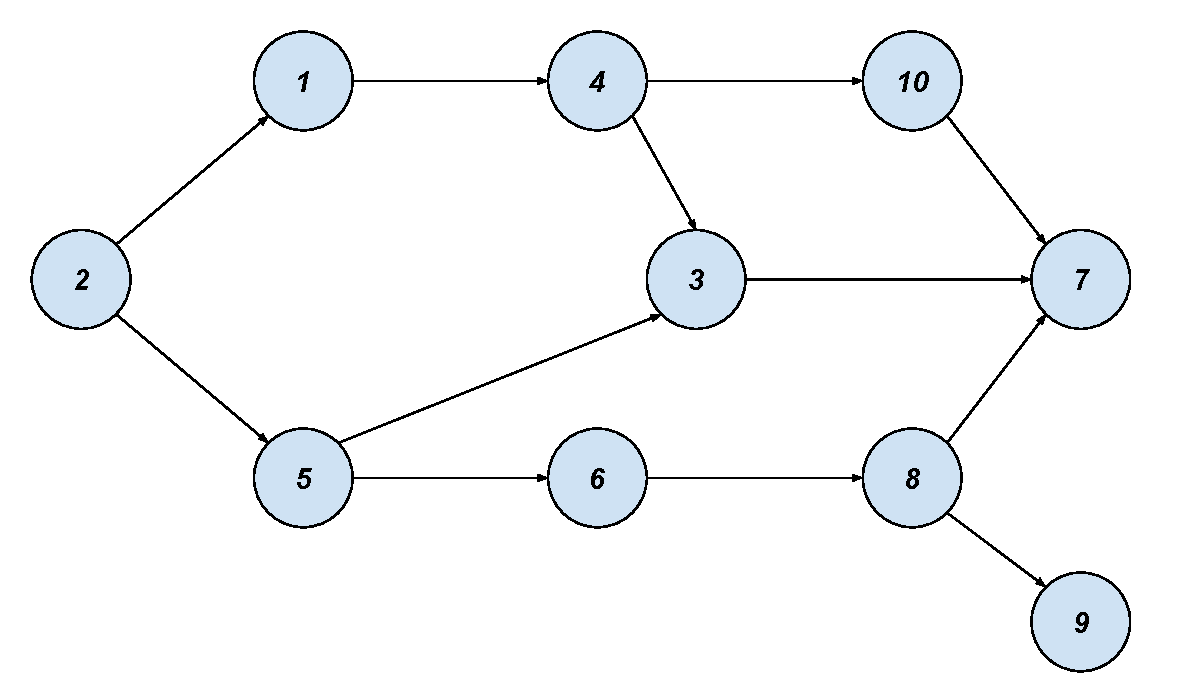
\includegraphics{graphs/floyd_warshall.pdf}
\end{figure}

$\mathfrak{D}_{ij}$ è l'insieme di tutti i cammini tra $i$ e $j$. \\
$\mathfrak{D}_{27} = \{\,<2,1,4,10,7>,\,<2,1,4,3,7>,\, <2,5,3,7>,\, <2,5,6,8,7>\}$

$\mathfrak{C}_{27}^{(1)} = \emptyset$ \\
$\mathfrak{C}_{27}^{(2)} = \emptyset$ \\
$\mathfrak{C}_{27}^{(3)} = \emptyset$ \\
$\mathfrak{C}_{27}^{(4)} = \{<2,1,4,3,7>\}$ (Cammino minimo e unico)\\
$\mathfrak{C}_{27}^{(5)} = \{<2,1,4,3,7>,\, <2,5,3,7>\}$ \\
Quindi $\mathfrak{C}_{ij}^{(n)} = \mathfrak{D}$ \\

\paragraph{Codice}

\lstinputlisting{code/floyd_warshall.txt}
Complessità : $\Theta(n^3)$

\[
W = D^0 =
 \begin{pmatrix}
  0 & 3 & 8 & \infty & -4 \\
  \infty & 0 & \infty & 1 & 7 \\
  \infty & 4 & 0 & \infty & \infty \\
  2 & \infty & -5 & 0 & \infty \\
  \infty & \infty & \infty & 6 & 0
 \end{pmatrix}
\]

\[
D^1 =
 \begin{pmatrix}
  0 & 3 & 8 & \infty & -4 \\
  \infty & 0 & \infty & 1 & 7 \\
  \infty & 4 & 0 & \infty & \infty \\
  2 & 5 & -5 & 0 & -2 \\
  \infty & \infty & \infty & 6 & 0
 \end{pmatrix}
\]

\[
D^2 =
 \begin{pmatrix}
  0 & 3 & 8 & 4 & -4 \\
  \infty & 0 & \infty & 1 & 7 \\
  \infty & 4 & 0 & 5 & 11 \\
  2 & 5 & -5 & 0 & -2 \\
  \infty & \infty & \infty & 6 & 0
 \end{pmatrix}
\]

\paragraph{Osservazioni}

\subparagraph{Osservazione A}

Se non ci sono cicli negativi, allora $\forall k,i = 1\ldots n, d_{ii}^{(k)} = 0$, ovvero ci sono solo valori nulli sulla diagonale principale.

\subparagraph{Dimostrazione per induzione su k}

Se $k=0$: VERO \\
Se $k>0$:

\begin{equation}
d_{ii}^{(k)} = min( \underbrace{d_{ii}^{(k-1)}}_\text{nullo per ipotesi} ,  \underbrace{d_{ik}^{(k-1)} + d_{ki}^{(k-1)}}_\text{positivo o nullo} ) = 0
\end{equation}

L'equazione risulta nulla poichè il primo termine $d_{ii}^{(k-1)}$ è nullo per ipotesi.
Il secondo termine non può essere negativo in quanto non ho cicli negativi.

\subparagraph{Osservazione B}

$\forall k = 1\ldots n,i,j \in V$

\[
\begin{cases} d_{ik}^{(k)} = d_{ik}^{(k-1)} \mbox{ Stessa colonna} \\ d_{kj}^{(k)} = d_{kj}^{(k-1)} \mbox{ Stessa riga} \end{cases}
\]

\subparagraph{Dimostrazione}

\begin{equation}
d_{ik}^{(k)} = min(  \underbrace{ d_{ik}^{(k-1)} , d_{ik}^{(k-1)}  }_\text{uguali} + \underbrace{ d_{kk}^{(k-1)} }_\text{nullo} ) = d_{ik}^{(k-1)}
\end{equation}

La stessa dimostrazione può essere applicata alla seconda equazione.

\subparagraph{Altre osservazioni}
Abbiamo notato che in caso appaia il valore \infty in una riga o in una colonna evidenziata, il valore delle altre celle non cambierà.

\subparagraph{Ottimizzazione}

Grazie alle osservazioni notiamo che possiamo utilizzare una sola matrice da sovrascrivere senza la necessità di averne una per ogni ciclo di $k$.

\lstinputlisting{code/floyd_warshall_sm.txt}

\chapter{Algoritmi Greedy}
Con algoritmi "greedy" intendiamo l'insieme degli algoritmi incapaci di capire la situazione complessiva, i quali prendono decisioni che sembrano migliori negli istanti di decisione. Ne fanno parte gli algoritmi di Kruskall, Prim e Dijkstra, i quali sono anche ottimali (ad eccezione di Dijkstra in caso di cicli negativi)

\paragraph{Ricerca di Maximum Clique}

Insieme di vertici completamente connesso da archi tra tutte le possibili coppie di vertici.

Una cricca massimale è una cricca che non può essere estesa includendo un altro vertice adiacente, cioè una cricca che non esiste esclusivamente dentro l'insieme dei vertici di una cricca più grande.

Una cricca massima è una cricca della dimensione più grande possibile in un dato grafo

\myworries{Manca grafo}

\lstinputlisting{code/greedy_clique.txt}

Complessità : $O(n^2 + nlog(n)) = O(n^2)$

\lstinputlisting{code/is_a_clique.txt}

Complessità : $O(n)$

Il problema della ricerca della Clique Massima è NP : non risolvibile in tempo polinomiale.

Notiamo però che ordinare secondo il numero di gradi non sempre funziona. Esempio:

\begin{figure}[H]
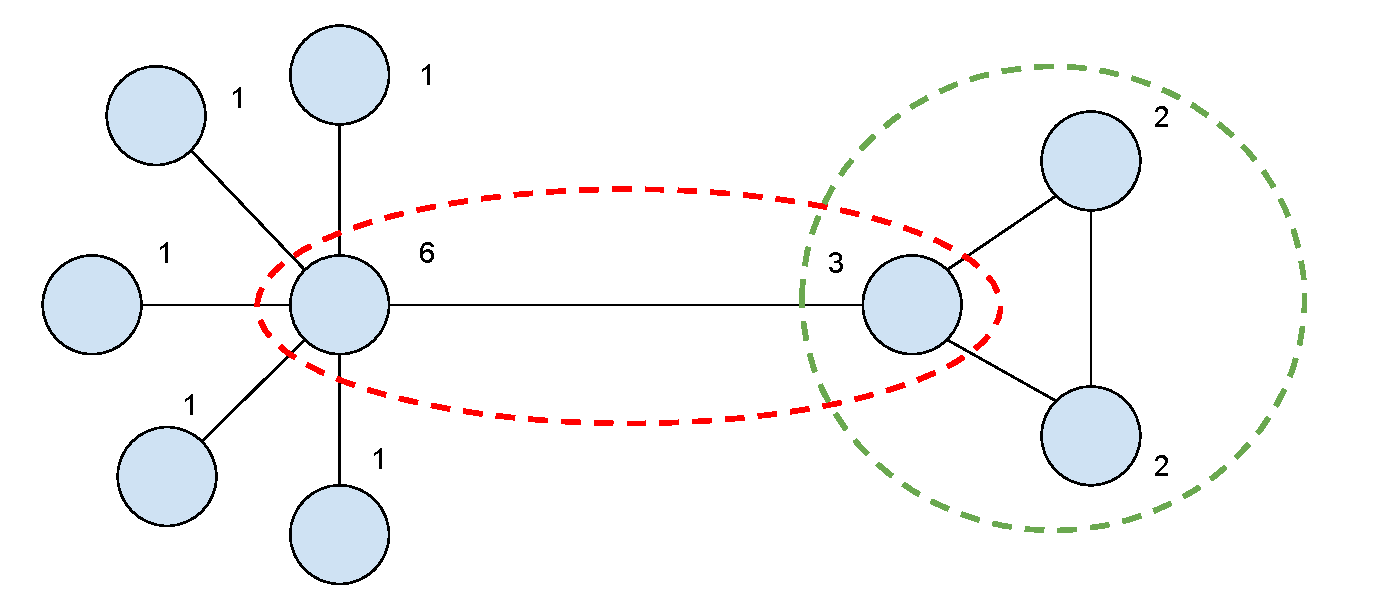
\includegraphics{graphs/greedy_grado.pdf}
\end{figure}

Sostituendolo con un ordinamento basato sul numero di triangoli incidenti non risolviamo prò il problema. Esempio:

\begin{figure}[H]
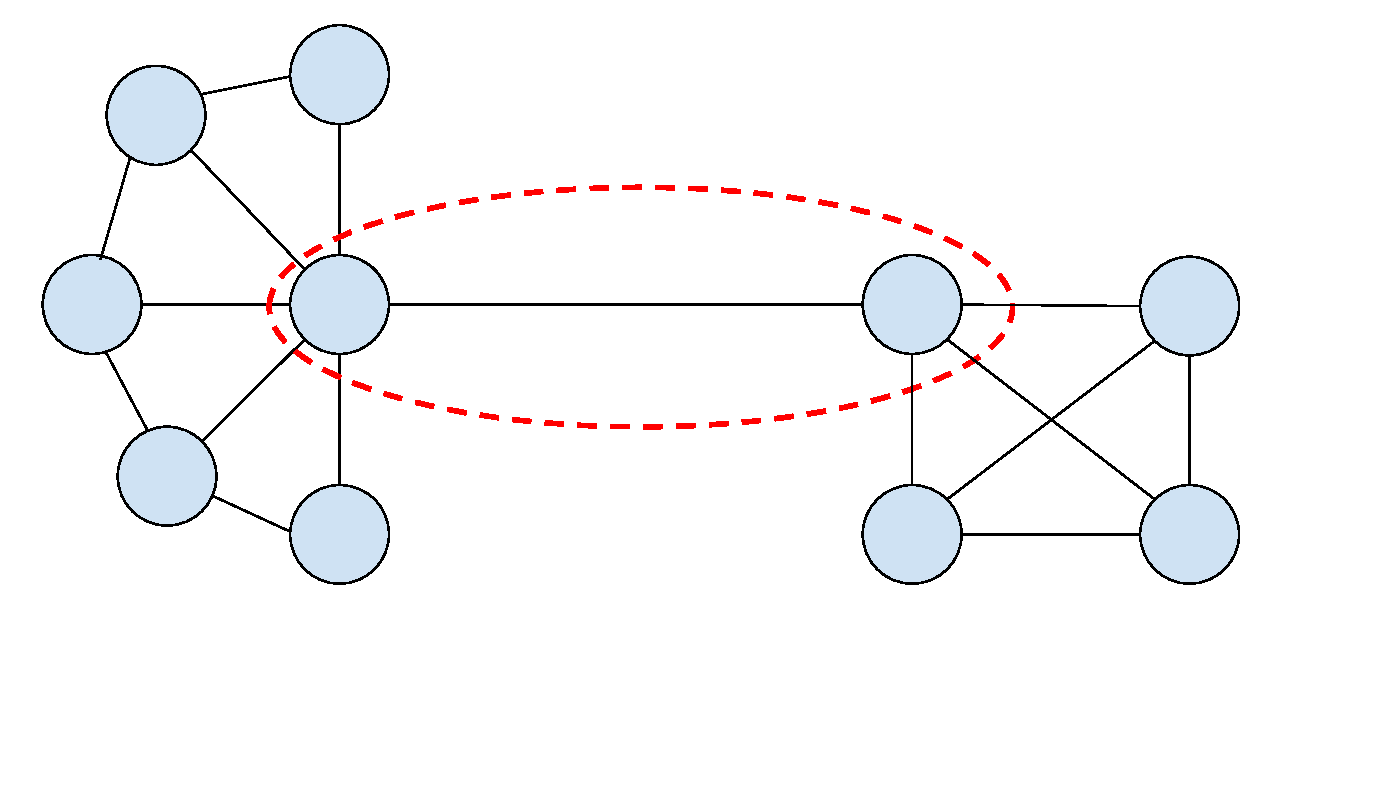
\includegraphics{graphs/greedy_triangoli.pdf}
\end{figure}

Notiamo che l'algoritmo è molto simile a Krusall. Non a caso infatti, tutti gli algoritmi Greedy han la stessa struttura:

\begin{enumerate}
\item Ordinamento
\item $ A \leftarrow \emptyset$
\item foreach $x$ (preso secondo ordinamento)
\item \hspace{\parindent} if $A \cup x$ è ok then
\item \hspace{\parindent} \hspace{\parindent} Aggiungi $x$ ad $A$
\end{enumerate}

\paragraph{Selezione attività}

Consideriamo un insieme di attività $t_1, t_2, \ldots , t_n$ con $t_i = (s_i, f_i)$ coppia in cui sono specificati i tempi di inizio e fine dell'attività. Esse sono rappresentabili attraverso un diagramma di Gantt.

\begin{ganttchart}[
x unit=0.22cm,
y unit title=0.5cm,
y unit chart=0.5cm,
title label font=\fontsize{4}{5}\selectfont,
bar label font=\tiny,
]{1}{48}
\ganttbar{Task 1}{1}{2} \\
\ganttbar{Task 2}{3}{7} \\
\ganttbar{Task 3}{8}{9} \\
\ganttbar{Task 4}{12}{15} \\
\ganttbar{Task 5}{3}{17} \\
\ganttbar{Task 6}{1}{12}
\end{ganttchart}

Vorremmo determinare un insieme di attività eseguibili in uno stesso momento, per farlo potremmo procedere all'ordinamento per:

\begin{enumerate}
\item Tempo di inizio
\item Tempo di fine
\item Durata
\end{enumerate}

Quale funzionerà meglio?


\chapter{NP Completezza}

Analizziamo la complessità ( o  "intrattabilità" ) di problemi:

Un problema $\mathcal{P} \subseteq \underbrace{\mathcal{I} }_\text{Istanze} x  \underbrace{\mathcal{S} }_\text{Soluzioni}$

Tipi di problemi:

\begin{enumerate}

\item Indecidibili: non esiste una soluzione algoritmica
\item Decidibili
\begin{enumerate}
\item Trattabili: quelli analizzati finora, tempo di esecuzione "ragionevole"
\item Intrattabili
\end{enumerate}

\end{enumerate}

\subsection{Esempio di algoritmo Indecidibile : Stop di Turing}

\myworries{Manca}

\subsection{Problemi decisionali e di ottimizzazione}

Un problema può essere di tipo decisionale se il tipo di output è booleano. Gli algoritmi studiati fino ad ora rientrano nella categoria dei problemi di ottimizzazione. Ci concentreremo ora sui problemi di tipo decisionale.

\subsection{Classi di complessità}

\subsubsection{Classe P}
Problemi risolvibili in tempo polinomiale

\begin{equation}
\{\mathcal{P} | \exists \text{ un algoritmo che risolve } \mathcal{P} \text{ in tempo polinomiale } O(n^k)\}
\end{equation}

\myworries{Manca schema}

\subsubsection{Classe NP}

\begin{equation}
\{\mathcal{P} | \exists \text{ un algoritmo di verifica per } \mathcal{P} \text{ di tempo polinomiale } O(n^k) \}
\end{equation}

\myworries{Manca schema}

\subsubsection{Complemento di un problema}

Il complemento $\mathcal{\overline{P}}$ del problema $\mathcal{P}$ è molto più complesso da calcolare in quanto, per verificarlo, si dovrebbero testare tutte le singole possibilità.

\myworries{Manca schema}

\subsubsection{Riducibilità polinomiale}

$\mathcal{P}_1 \underbrace{\leq_P}_\text{Riducibile polinomialmente} \mathcal{P}_2$ se esiste un algoritmo polinomiale che traforma ciascuna istanza de problema $\mathcal{P}_1$ in un'istanza del problema $\mathcal{P}_2$

\paragraph{Proprietà}

\myworries{Manca}

\subsubsection{Classe NPC - NP Completi}

\begin{equation}
\{\mathcal{P} | \mathcal{P} \in \text{ NP e } \forall \mathcal{P}' \in \text{ NP }, \mathcal{P}' \leq_P \mathcal{P} \}
\end{equation}

\myworries{Manca schema Venn}

\subsubsection{Teorema fondamentale dell'NP-Completezza}

\begin{equation}
P \cap NPC \neq \emptyset \Rightarrow P = NP
\end{equation}

\paragraph{Dimostrazione}

Ipotesi : $P \cap NPC \neq \emptyset$ \\
Tesi : $\text{P} = \text{NP}$ \\

Dimostrazione : 

\begin{enumerate}
\item $\text{P} \subseteq \text{NP}$, già dimostrata. OK
\item $\text{NP} \subseteq \text{P}$
\end{enumerate}

\myworries{Manca}


\backmatter

\end{document}
